%%%%%%%%%%%%%%%%%%%%%%%%%%%%%%%%%%%%%%%%%
% Masters/Doctoral Thesis
% LaTeX Template
% Version 3.0 (18/3/22)
%
% This template was downloaded from:
% http://www.LaTeXTemplates.com
%
% Version 2.x major modifications by:
% Vel (vel@latextemplates.com)

% Version 3.x modifications by:
% Felix Friese
%
% This template is based on a template by:
% Steve Gunn (http://users.ecs.soton.ac.uk/srg/softwaretools/document/templates/)
% Sunil Patel (http://www.sunilpatel.co.uk/thesis-template/)
%
% Template license:
% CC BY-NC-SA 3.0 (http://creativecommons.org/licenses/by-nc-sa/3.0/)
%
%%%%%%%%%%%%%%%%%%%%%%%%%%%%%%%%%%%%%%%%%

%----------------------------------------------------------------------------------------
%	PACKAGES AND OTHER DOCUMENT CONFIGURATIONS
%----------------------------------------------------------------------------------------


%\RequirePackage{standalone}
\RequirePackage{sectsty}        % make section heading sans-serif
\RequirePackage{fontawesome5}
\RequirePackage[utf8]{inputenc} % Required for inputting international characters
\RequirePackage[T1]{fontenc} % Output font encoding for international characters
\RequirePackage{mathpazo} % Use the Palatino font by default
\RequirePackage[mathscr]{eucal}
\RequirePackage{microtype}  % somehow make stuff look nicer
\microtypesetup{nopatch=item} % somehow needed
\RequirePackage[backend=bibtex,citestyle=numeric, bibstyle=ieee,natbib=true,sorting=ynt]{biblatex} % Use the bibtex backend
\addbibresource{references.bib} % The filename of the bibliography

\AtEveryBibitem{
    \clearfield{urlyear}
    \clearfield{urlmonth}
    \clearfield{urldate}
}

\RequirePackage{comment}  % comment out sections
% ------------------
% align equations
% ------------------
\RequirePackage{amsmath}  % align equations

%MATHSYMB
\RequirePackage{amssymb}

% ------------------
% wrap figure in text blocks
% ------------------
\RequirePackage{wrapfig}

% ------------------
% fancy plots
% ------------------
\RequirePackage{pgfplots}
\usetikzlibrary{calc, shapes, fit, positioning, arrows.meta, matrix, pgfplots.groupplots}
\usepgfplotslibrary{fillbetween}%, external}
%\tikzexternalize

% use `compat' level 1.3 (or higher) to use the advanced placement features for the axis labels
\pgfplotsset{
    compat=newest
}
% ------------------
% floating stuff, captions and subcaptions, idk
% ------------------
\RequirePackage{float}
\RequirePackage{subcaption}

% ------------------
% very important lorem ipsum package
% ------------------
\RequirePackage{lipsum}

% ------------------
% remark environment
% ------------------
\RequirePackage{amsthm}
\newtheorem*{remark}{Remark}

% ------------------
% code sections
% ------------------
\RequirePackage{fontspec}
\setmonofont{JetBrainsMono}[
Path=./JetbrainsFontFiles/,
Scale=0.85,
Extension = .ttf,
UprightFont=*-Regular,
BoldFont=*-Bold,
ItalicFont=*-Italic,
BoldItalicFont=*-BoldItalic
]
\RequirePackage{minted}



\RequirePackage[autostyle=true]{csquotes} % Required to generate language-dependent quotes in the bibliography



\usemintedstyle{manni}
%----------------------------------------------------------------------------------------
%    COLORS
%----------------------------------------------------------------------------------------
\definecolor{LightGray}{gray}{0.95}
\definecolor{green}{rgb}{0,0.7,0}
\definecolor{modernblue}{HTML}{224fa4}
\definecolor{pyratesdarkred}{HTML}{9f294e}
\definecolor{pyratesgreen}{HTML}{3d734f}
\definecolor{pyratesorange}{HTML}{c76d00}
\definecolor{pyratespurple}{HTML}{473579}


% ------------------
% section number depths
% ------------------
\setcounter{tocdepth}{2}
\setcounter{secnumdepth}{3}

\allsectionsfont{\sffamily}

%----------------------------------------------------------------------------------------
%	MARGIN SETTINGS
%----------------------------------------------------------------------------------------

\geometry{
	paper=a4paper, % Change to letterpaper for US letter
	inner=2.5cm, % Inner margin
	outer=3.8cm, % Outer margin
	bindingoffset=.5cm, % Binding offset
	top=1.5cm, % Top margin
	bottom=1.5cm, % Bottom margin
	%showframe, % Uncomment to show how the type block is set on the page
}

%----------------------------------------------------------------------------------------
%	THESIS INFORMATION
%----------------------------------------------------------------------------------------

% Your thesis title, this is used in the title and abstract, print it elsewhere with \ttitle
\thesistitle{Simulating sedation-induced unconsciousness in a Neural-Mass-Model}
%to improve algorithms for state-of-consciousness detection in patients in the Minimally Conscious State

% Your supervisor's name, this is used in the title page, print it elsewhere with \supname
\supervisor{Dr. Malte \textsc{Schilling}}

% Your examiner's name, this is not currently used anywhere in the template, print it elsewhere with \examname
\examiner{Prof Dr. Helge \textsc{Ritter}}
% Your degree name, this is used in the title page and abstract, print it elsewhere with \degreename
\degree{Master of Science}
% Your name, this is used in the title page and abstract, print it elsewhere with \authorname
\author{Felix \textsc{Friese}}


% Your subject area, this is not currently used anywhere in the template, print it elsewhere with \subjectname
\subject{Intelligent Systems}
% Keywords for your thesis, this is not currently used anywhere in the template, print it elsewhere with \keywordnames
\keywords{EEG, NMM, GABA-A, Propofol, Anaesthesia}
% print it elsewhere with \univname
\university{\href{https://uni-bielefeld.de/}{Bielefeld University}}
% print it elsewhere with \deptname
\department{\href{https://www.uni-bielefeld.de/technische-fakultaet/}{Faculty of Technology}}
% print with \groupname
\group{\href{https://www.uni-bielefeld.de/fakultaeten/technische-fakultaet/forschung/ag-ueberblick/neuroinformatik/}{Neuroinformatics Group}}
%print with \facname
\faculty{\href{https://www.uni-bielefeld.de/technische-fakultaet/}{Faculty of Technology}}

\AtBeginDocument{
\hypersetup{pdftitle=\ttitle} % Set the PDF's title to your title
\hypersetup{pdfauthor=\authorname} % Set the PDF's author to your name
\hypersetup{pdfkeywords=\keywordnames} % Set the PDF's keywords to your keywords
}

\DeclareSIUnit{\molar}{M}

%\usepackage{scrhack}
\RequirePackage{tikz}

\RequirePackage{linegoal}

\RequirePackage{import}
\newcommand\iltodo[1]{
\fcolorbox{orange}{orange!10}{
    \fcolorbox{black}{yellow!70}{\small\faIcon{tasks}~ \texttt{Todo}}
    \hspace{4pt} \texttt{#1}}
}

\newcommand\todo[1]{\par
\noindent\fcolorbox{orange}{orange!10}{\parbox{\linegoal}{
    \fcolorbox{black}{yellow!70}{\small\faIcon{tasks}~ \texttt{Todo}}
    \hspace{4pt} \texttt{#1}}}~\\
}

\newcommand\question[1]{\par
\noindent\fcolorbox{yellow}{yellow!10}{\parbox{\linegoal}{
    \fcolorbox{black}{yellow!70}{\small\faIcon{question}~ \texttt{Question}}
    \hspace{4pt} \texttt{#1}}}~\\
}

\newcommand\incomplete[1]{\par
\noindent\fcolorbox{red}{red!10}{\parbox{\linegoal}{
    \fcolorbox{black}{orange!70}{
        \small\faIcon{exclamation-triangle}~\texttt{Section Incomplete}
    }
\texttt{#1}}}~\\[1em]}


\newcommand{\newremark}[2]{

    \vspace{1em}\par
    \noindent\fcolorbox{yellow}{yellow!10}{
       \begin{minipage}{\linewidth}
        \textbf{Remark} (#1). \textit{ #2 }
       \end{minipage}
    }

    \vspace{1em}\noindent
}

\newcommand{\newremarkimg}[3]{

    \vspace{1em}
    \noindent\fcolorbox{yellow}{yellow!10}{
       \begin{minipage}{\linewidth}
           #2
        \textbf{Remark} (#1). \textit{ #3 }
       \end{minipage}
    }

    \vspace{1em}\noindent
}

\newcommand\citationneeded{\textcolor{blue}{[citation-needed]}}

\begin{document}

\frontmatter % Use roman page numbering style (i, ii, iii, iv...) for the pre-content pages

\pagestyle{plain} % Default to the plain heading style until the thesis style is called for the body content

%----------------------------------------------------------------------------------------
%	TITLE PAGE
%----------------------------------------------------------------------------------------

\begin{titlepage}
\begin{center}

\vspace*{.06\textheight}
{\scshape\LARGE \univname\par}\vspace{1.5cm} % University name
\textsc{\Large Masters Thesis}\\[0.5cm] % Thesis type

\HRule \\[0.4cm] % Horizontal line
{\huge \bfseries \ttitle\par}\vspace{0.4cm} % Thesis title
\HRule \\[1.5cm] % Horizontal line

\begin{minipage}[t]{0.4\textwidth}
\begin{flushleft} \large
\emph{Author:}\\
\href{}{\authorname} % Author name
\end{flushleft}
\end{minipage}
\begin{minipage}[t]{0.4\textwidth}
\begin{flushright} \large
\emph{Supervisor:} \\
\href{https://ni.www.techfak.uni-bielefeld.de/people/mschilli}{\supname} % Supervisor name

\vspace*{.04\textheight}

\emph{Examiner:} \\
\href{https://ni.www.techfak.uni-bielefeld.de/people/helge}{\examname} % Examiner name
\end{flushright}
\end{minipage}\\[3cm]

\vfill

\large \textit{A thesis submitted in fulfillment of the requirements\\ for the degree of \degreename}\\[0.3cm] % University requirement text
\textit{in the}\\[0.4cm]
\groupname\\\deptname\\[2cm] % Research group name and department name

\vfill

{\large \today}\\[4cm] % Date
%\includegraphics{Logo} % University/department logo - uncomment to place it

\vfill
\end{center}
\end{titlepage}

%----------------------------------------------------------------------------------------
%	DECLARATION PAGE
%----------------------------------------------------------------------------------------

% 
\begin{declaration}
	\addchaptertocentry{\authorshipname} % Add the declaration to the table of contents
	\noindent I, \authorname, declare that this thesis titled, \enquote{\ttitle} and the work presented in it are my own. I confirm that:
	
	\begin{itemize} 
		\item Where any part of this thesis has previously been submitted for a degree or any other qualification at this University or any other institution, this has been clearly stated.
		\item Where I have consulted the published work of others, this is always clearly attributed.
		\item Where I have quoted from the work of others, the source is always given. With the exception of such quotations, this thesis is entirely my own work.
		\item I have acknowledged all main sources of help.
		\item Where the thesis is based on work done by myself jointly with others, I have made clear exactly what was done by others and what I have contributed myself.\\
	\end{itemize}
	
	\noindent Signed:\\
	\rule[0.5em]{25em}{0.5pt} % This prints a line for the signature
	
	\noindent Date:\\
	\rule[0.5em]{25em}{0.5pt} % This prints a line to write the date
\end{declaration}

\cleardoublepage


%----------------------------------------------------------------------------------------
%	QUOTATION PAGE
%----------------------------------------------------------------------------------------

% \vspace*{0.2\textheight}

% \noindent\enquote{\itshape
% It is surely important that the differences between coma, deep sleep,
% being under anesthesia, on the one hand, and being alert on the other,
% all involve changes in the brain.}\bigbreak

% \hfill Patricia Churchland

%----------------------------------------------------------------------------------------
%	ABSTRACT PAGE
%----------------------------------------------------------------------------------------

\begin{abstract}
\addchaptertocentry{\abstractname} % Add the abstract to the table of contents
\todo{This is old! Re-write the abstract to match the new hypothesis! (very last thing to do)}
\textcolor{gray}{\textit{Patients with severe Traumatic Brain Injuries (TBI) often remain in a state of unresponsive
wakefulness.
Brain-Computer-Interface (BCI)-based systems promise to improve the state assessment and to open a
communication channel for patients to express their intent while in conscious states.
Developing such a BCI-System (e.g., with EEG), including the necessary algorithms to assess a patients current
wakefulness or consciousness state from EEG data is a challenging task.
Development, testing and evaluation of these algorithms requires labeled data (ground truth),
which is almost impossible to obtain given the patients' lack of communication capabilities.
Therefore, it would be desirable to generate a synthetic signal, which should ideally resemble
real EEG data in all relevant features.
We previously developed a simple ICA-based model, which generates a multichannel EEG from base-signals with
configurable spectral features.
While this proved useful for testing numerous components of our signal-analysis framework,
it lacks biological plausibility and explanatory power to model the changes in the signal's
properties given an altered state of consciousness.
In this thesis, we propose an approach towards overcoming these issues while sticking with the original goal of
generating realistic, practically useful surrogate data.
A biologically motivated Neural Mass Model (NMM) on cortical-column level is implemented,
which is able to approximate the effects of sedation-induced unconsciousness on the generated signal.
The model is then shown to be able to reproduce the characteristic effects
that sedation has on the EEG-Signals of real subjects.
This is a first step to a model of consciousness-altering processes in the brain,
which could ultimately be extended to realistically simulate other processes like sleep and trauma-induced DoC,
facilitating better detection algorithms and furthering the goal to develop working BCI-Systems in the given context.}}
\end{abstract}

%----------------------------------------------------------------------------------------
%	ACKNOWLEDGEMENTS
%----------------------------------------------------------------------------------------

%\begin{acknowledgements}
%\addchaptertocentry{\acknowledgementname} % Add the acknowledgements to the table of contents
%The acknowledgements and the people to thank go here, don't forget to include your project advisor\ldots
%\end{acknowledgements}

%----------------------------------------------------------------------------------------
%	LIST OF CONTENTS/FIGURES/TABLES PAGES
%----------------------------------------------------------------------------------------
\hypersetup{linkcolor=black}{
    \tableofcontents % Prints the main table of contents
 %   \listoffigures % Prints the list of figures
 %   \listoftables % Prints the list of tables
}
%----------------------------------------------------------------------------------------
%	ABBREVIATIONS
%----------------------------------------------------------------------------------------
\begin{abbreviations}{ll} % Include a list of abbreviations (a table of two columns)

\textbf{BCI} & \textbf{B}rain \textbf{C}omputer \textbf{I}nterface\\
\textbf{DoC} & \textbf{D}isorder(s) \textbf{o}f \textbf{C}onsciousness\\
\textbf{EEG} & \textbf{E}lectro\textbf{e}ncephalo\textbf{g}raphy\\
\textbf{fMRI} & \textbf{f}unctional \textbf{M}agnetic \textbf{R}esonance \textbf{I}maging\\
%\textbf{EIN} & \textbf{E}xcitatory \textbf{I}nter\textbf{n}euron\\
%\textbf{EPSP} & \textbf{E}xcitatory \textbf{P}ost-\textbf{S}ynaptic-\textbf{P}otential\\
\textbf{GA} & \textbf{G}eneral \textbf{A}naesthesia\\
\textbf{GABA} & \textbf{G}amma-\textbf{A}mino\textbf{b}utyric \textbf{A}cid\\
\textbf{ICA} & \textbf{I}ndependent \textbf{C}omponent \textbf{A}nalysis\\
\textbf{[E/I]IN} & [\textbf{E}xcitatory/\textbf{I}nhibitory] \textbf{I}nter\textbf{n}euron\\
%\textbf{IIN} & \textbf{I}nhibitory \textbf{I}nter\textbf{n}euron\\
%\textbf{IPSP} & \textbf{I}nhibitory \textbf{P}ost-\textbf{S}ynaptic-\textbf{P}otential\\
\textbf{[L/R]OC} & [\textbf{L}oss/\textbf{R}ecovery] \textbf{O}f \textbf{C}onsciousness\\
\textbf{NMM} & \textbf{N}eural \textbf{M}ass \textbf{M}odel\\
\textbf{PC} & \textbf{P}yramidal \textbf{C}ell\\
\textbf{PSD} & \textbf{P}ower \textbf{S}pectral \textbf{D}ensity\\
\textbf{[E/I]PSP} & [\textbf{E}xcitatory/\textbf{I}nhibitory] \textbf{P}ost-\textbf{S}ynaptic-\textbf{P}otential\\
\textbf{TBI} & \textbf{T}raumatic \textbf{B}rain \textbf{I}njury\\

\end{abbreviations}


%----------------------------------------------------------------------------------------
%	THESIS CONTENT - CHAPTERS
%----------------------------------------------------------------------------------------

\mainmatter % Begin numeric (1,2,3...) page numbering

\pagestyle{thesis} % Return the page headers back to the "thesis" style

% Include the chapters of the thesis as separate files from the Chapters folder

\chapter{Introduction}\label{ch:introduction}





\section{Motivation}\label{sec:motivation}
%%%%%%%%%%%%%%%%%%%%%%%%%%%%%%%%%%%%%%%%%%%%%%%%%%%%%%%%%%%%%%%
% How do states of consciousness change? How are they defined %
%%%%%%%%%%%%%%%%%%%%%%%%%%%%%%%%%%%%%%%%%%%%%%%%%%%%%%%%%%%%%%%
The highly complex processes of changing states of consciousness in the human brain are still barely understood.
States of consciousness have historically been defined based on behavioral observations such as responsiveness to
stimuli.
As no other indications, save simple physiological measurements such as pulse and respiration rate,
were available, the concept of awareness was tightly linked to observable behavior.
While the great majority of medical applications to determine levels of consciousness,
even in practical clinical contexts~\cite{jain_glasgow_2022},
are still covered by these observations,
there are cases in which the link between consciousness and displayed behavior falls apart;
striking examples are some disorders of consciousness (DOC) as well as the total locked-in
syndrome~\cite{bauer_varieties_1979},
where patients are unable to display any visible behavior,
while maintaining some or even full awareness.
Although cases like these are rare, they highlight that consciousness needs to be studied at its source -- on the
level of brain-activity -- to fully understand the mechanisms that lead to its different states.
%
% Additionally, some edge-cases surrounding DOCs may require changes to common state-definitions,
% that are based on [...]
%
%%%%%%%%%%%%%%%%%%%%%%%%%%%%%%%%%%%%%%
% How can we measure brain-activity? %
%%%%%%%%%%%%%%%%%%%%%%%%%%%%%%%%%%%%%%
Brain-activity can be measured directly or indirectly.
Direct measurement with electrodes in the brain, while more accurate,
poses the obvious problem of its invasive nature and faces the challenge of realistically\todo{rephrase} only allowing very
localized measurements \textcolor{blue}{[citation needed]}.
Various neuroimaging techniques, which indirectly measure brain-activity, have been used to study levels of
awareness since their emergence.
Already in the 1880`s, Angelo Mosso measured scalp-pulse variations in subjects
with skull-injuries during challenging tasks,
and concluded an increased blood-flow to the brain~\cite{mosso_ueber_1881}.
Improved techniques like the fMRI and the EEG allow for non-invasive observation of brain-activity and have been
used extensively to study the dynamics of the brain during sleep and loss and return of consciousness
\textcolor{blue}{[citation needed]}.
Some phenomena, like predictable changes in signal-frequencies and some critical brain regions involved in
consciousness-modulation have been identified and are well documented \textcolor{blue}{[citation needed]}.
Techniques to measure levels of consciousness via neuroimaging have been proposed~\cite{sigl_introduction_1994,
    casali_theoretically_2013} and used in practise~\cite{mathur_bispectral_2022}.
However, exact mechanisms behind state-changes are still object of fundamental research.

%%%%%%%%%%%%%%%%%%%%%%%%%%%%%%%%%%%%%%%%%%%%%%%
% How to study state-changes most efficently? %
%%%%%%%%%%%%%%%%%%%%%%%%%%%%%%%%%%%%%%%%%%%%%%%
Controlled state-changes, like inducing loss-of-consciousness with anaesthetic drugs,
are exceptionally well-suited for studying the underlying mechanisms of consciousness,
as they allow for repeatable conditions.
Furthermore, the neuro-chemical mechanisms of the drugs provide a good starting-point for modeling these processes.
The sedative propofol is the most commonly used drug to induce controlled loss of consciousness
during general anaesthesia.
Propofol's neuro-chemical mode of action and its specific effects on synaptic receptors are well understood,
which lays a solid foundation to study the brain-dynamics associated with loss of consciousness.

A promising approach to further our insights step by step, is to simulate controlled state-changes
(such as anaesthesia) in computer-models to develop an understanding of the dynamics of brain-activity and its
effects on consciousness. %% controlled induction/loss of consciousness to directly test hypothesis experimentally
Computer-models of the brain (or parts of it) exist on different levels~\cite{panahi_generative_2021},
including simulations of individual neurons and population-based approaches.
Neural-Mass-Models (NMMs), members of the latter, model synaptic connections between populations of different types
of neurons and have proven to replicate multiple abstract phenomena of brain-dynamics\cite{bojak_neural_2014,
    knösche_jansen-rit_2014} within a small cortical
column.
The simplifications they provide allow efficient real-time simulation of signals,
while preserving many important characteristics of EEG or MEG signals.

\todo{improve explanation of NMMs}

By combining the well-known properties of propofol with an NMM, we can hope to gain insights into the mechanisms that
govern changes of brain-dynamics in the presence of consciousness-altering drugs.
While the abstract nature of NMMs, along with its limitations must always be
considered~\cite{deschle_validity_2021},
the results of simulated experiments can provide valuable research indications.


One of the most commonly used models in the area of neural population models is the
Jansen-Rit~\cite{jansen_electroencephalogram_1995} (JR) NMM,
which is based on efforts by Wilson \& Cowan~\cite{wilson_excitatory_1972},
Lopes da Silva et al.~\cite{lopes_da_silva_model_1974, lopes_da_silva_models_1976} and
Zetterberg et al.~\cite{zetterberg_performance_1978}.
It is one of the most simple and basic population models,
while retaining `a considerable degree of biological realism` and
`producing a surprisingly rich repertoire of dynamic behaviors`~\cite{knösche_jansen-rit_2014}.
Many efforts in the field are based on the JR NMM, e.g.~\cite{wendling_relevance_2000, david_neural_2003,
    moran_dynamic_2009, spiegler_bifurcation_2010, cona_thalamo-cortical_2014, bensaid_coalia_2019} and others.



Neural-Mass models have been widely used to simulate the properties of different states of consciousness.
Cona et al.~\cite{cona_thalamo-cortical_2014} adapted the JR NMM to simulate effects
of different stages of sleep.
Their model accounts for thalamo-cortical modulation of cortico-cortical connectivity as an important mechanism to
influence these transitions.
Bensaid et al.'s COALIA Framework~\cite{bensaid_coalia_2019},
makes use of a similar structure, while using over 60 interconnected NMM-modules and applying a
transformation onto scalp electrodes using a realistic head-model with tissue conductivities.

% steyn_ross_sleep_2005
As we are looking to simulate propofol-induced unconsciousness, similar approaches bear special consideration:
To simulate phenomena specific to general anaesthesia,
Steyn-Ross et al.~\cite{steyn_ross_modelling_2004, hutt_progress_2011} developed a model based
on Liley et al.'s continuum model~\cite{liley_continuum_1999}.
\todo{short explanation of continuous cortical field theories CFT, the difference to `normal' NMMs}

This work aims to use a non-CFT approach based on the JR model and evaluate if it is able to reproduce the
behavior observed in Steyn-Ross et al.'s CFT model ~\cite{hutt_progress_2011}.
While the basic JR model is able to produce rich patterns of dynamic behavior~\cite{spiegler_bifurcation_2010},
large regions of its parameter-space generate sinusoidal signals with a single pronounced frequency,
which might limit its ability to reproduce the expected phenomena (as noted by~\cite{kuhlmann_neural_2016}).
Therefore, the subpopulation-extension proposed by David \& Friston~\cite{david_neural_2003} is also employed to
produce a more realistic baseline frequency spectrum.

%\cite{luppi_paths_2021}}
%
%Liang et al.~\cite{liang_pharmacokinetics-neural_2015} focussed on relating propofol-induction to effect-site
%concentration, which is an important parameter in any model for anaesthesia-simulation.

%
%\section{Collection of Quotes}
%
%'Although our understanding of the actions of propofol at the molecular level is quite extensive,
%we do not entirely understand how these molecular effects translate into alterations in cellular,
%synaptic and neural network function, and in turn cause unconsciousness [88].
%This knowledge gap is, at least in part, the result of a lack of a generally accepted theory of consciousness.
%In recent years, cognitive neuroscience has seen a resurgence of interest in this topic,
%with attempts to integrate anaesthesia and sleep research in order to address this deficiency.
%This resurgence has revealed several brain areas that play a crucial role in generation of consciousness,
%and which are extensively influenced by hypnotic drugs.'
%\cite{sahinovic_clinical_2018}\\[1em]



% Chapter Template

\chapter{Technical Concepts}\label{ch:technical-concepts} % Main chapter title

%
\section{States of Consciousness}

\subsection{Definition}
    \qquad \todo{which states of consciousness are commonly defined}
\subsection{State Transitions}
\subsubsection{Natural Transitions}
    \qquad \qquad \todo{how states transition into each other naturally}
\subsubsection{Sedation}
    \qquad \qquad \todo{how sedation differs from natural loss of consciousness}
\subsection{Disorders of Consciousness}
    \qquad \todo{the symptoms of DOCs}
% \begin{itemize}
%	\item How do we define States of Consciousness?
%	\item What do we know about them (and what do we not)?
%	\begin{itemize}
%		\item How do these states change (naturally)?
%		\item What has an influence on the state?
%		\item What happens for DOCs?
%	\end{itemize}
% \end{itemize}



%\pagebreak
\section{General Anaesthesia}\label{sec:general-anaesthesia}
Having established the theoretical background for our models,
we can approach~\ref{goal:implement_propofol} by investigating the effects of propofol in the context of anaesthesia.
GA is usually employed in surgical contexts to keep patients from experiencing pain during medical
procedures, e.g., an operation.
Sedative drugs are carefully administered to the patient by trained practitioners to induce loss of consciousness,
without causing permanent damage to the brain or other parts of the body.
Propofol is the most popular sedative for GA~\cite{miner_clinical_2007, sahinovic_clinical_2018}
and its effects on the brain have been extensively studied,
which makes it a good candidate for our simulation goals.

\subsubsection{Realistic propofol concentrations during GA}\label{subsubsec:realistic-prop-conc-during-ga}
To estimate sensible parameter ranges for our model,
it is helpful to establish realistic dosages of propofol in clinical practice.
Some works (e.g,~\cite{iwakiri_individual_2005, ferreira_patterns_2020}) state propofol concentrations in $\SI{}{\frac{\micro\gram}{\milli\litre}}$,
while others (e.g.,~\cite{kitamura_effects_2003, mcdougall_propofol_2008}) report values in $\SI{}{\micro\molar}$ (micromolar =
$\SI{}{\frac{\micro\mol}{\litre}}$).
To get comparable numbers, we first need to establish the following relation for propofol
(molar mass: $\SI{178.27}{\gram}$):
\[ \SI{1}{\frac{\micro\gram\hspace{0.5em}\text{\tiny{Propofol}}}{\milli\litre}}  =
\frac{ \SI{1}{\frac{\micro\gram}{\milli\litre}}}{\SI{178.27}{\frac{\gram}{\mol}}} \approxeq \SI{5.609}{\micro\molar} \]
In this work, we will use $\SI{}{\micro\molar}$ as our default unit
but additionally provide original values in $\SI{}{\frac{\micro\gram}{\milli\litre}}$ where they are taken from a source.

Effect-site concentrations ($c_{e}$, concentration near the synaptic receptors) of propofol may easily range
up to $\SI{5}{\frac{\micro\gram}{\milli\litre}} (\approx\SI{28}{\micro\molar})$.
Loss of consciousness (LOC) occurs on average at $c_e \sim\SI{2.0}{\frac{\micro\gram}{\milli\litre}} (\approx\SI{11
.2}{\micro\molar})$,
while the recovery of consciousness (ROC) averages at $c_e \sim\SI{1.8}{\frac{\micro\gram}{\milli\litre}}
(\approx\SI{10.1}{\micro\molar})$.
Both values may vary substantially for individual subjects.
LOC has a strong tendency to occur at higher concentrations than ROC.~\cite{iwakiri_individual_2005,
    ferreira_patterns_2020}
Throughout GA, effect-site concentration is commonly derived from measured
blood-plasma concentration ($c_p$) using more or less complex Pharmacokinetic (PK)-Models
(e.g.,~\cite{eleveld_general_2014, liang_pharmacokinetics-neural_2015}),
as direct measurement of $c_{e}$ in the brain is impractical for obvious reasons.
As our model requires the concentration at the receptors, it will use $c_{e}$ directly, however,
the role of PK-Models with respect to reported effect-site concentrations in many works is crucial
and important to acknowledge.


\subsubsection{Effects of propofol on the inhibitory PSP}
Propofol is a GABA\textsubscript{A} receptor agonist, i.e, it potentiates the effect of inhibitory
GABA neurotransmitters at GABA\textsubscript{A} receptors and thereby modulates
the IPSP~\cite{sahinovic_clinical_2018}.
Research on the effect of propofol on the IPSC (Inhibitory Post-Synaptic Current) and EPSC
of cortical neurons has shown that propofol strongly affects the IPSP decay time.
The EPSP and the amplitude of the IPSP of these neurons are unaffected by propofol.
Effect-site concentrations at clinically relevant levels increase the IPSP decay time
significantly (e.g., around $\SI{10}{\micro\molar}$ the decay time roughly doubles).
\cite{kitamura_effects_2003, mcdougall_propofol_2008}


\subsubsection{Biphasic Effect}\label{subsubsec:biphasic-effect}
A biphasic effect (an initial increase of an effect, that decreases with higher concentrations) in the EEG can be
observed for many sedatives.
At low drug-concentrations during induction (and roughly during loss of consciousness)
there are surges of brain-activity,
which disappear with further increase of the dosage and the onset of the comatose state.
Similar observations have been made during the recovery of consciousness,
when the steadily declining levels of the anaesthetic agent temporarily cause pronounced brain-activity before the
subject fully regains consciousness.
For propofol, a temporary steep increase in EEG amplitude,
loosely correlated with the onset of LOC, as well as ROC can be observed.
\cite{kuizenga_quantitative_1998, kuizenga_biphasic_2001}
% Stage-transition, unstable area between two stable states (consciousness/unconsciousness)


\subsubsection{Hysteresis of propofol}\label{subsubsec:hysteresis}

If the state of a system depends not only on its parameters, but also the systems' history,
this dependency is called hysteresis.
The human body often reacts differently to the same concentration of a drug,
depending on whether the concentration is rising or decaying.
Hysteresis is well documented during propofol-induced GA~\cite{kuizenga_quantitative_1998,
    iwakiri_individual_2005,sepulveda_evidence_2018,ferreira_patterns_2020, su_hysteresis_2020}.
The most prominent effect is a counter-clockwise hysteresis for LOC and ROC (as mentioned
in~\ref{subsubsec:realistic-prop-conc-during-ga});
The loss on responsiveness of subjects usually start at higher concentrations than its return.
While some of that effect might be caused by inaccurate PK-Models,
misgauging the actual effect-site concentration,
there is a growing body of research supporting the notion of neural inertia
(the brain's resistance to state changes)~\cite{su_hysteresis_2020, ferreira_patterns_2020, luppi_inert_2021}.
Nonetheless, doubts remain with respect to the origin
of the observed time-lag~\cite{mckay_pharmacokinetic_pharmacodynamic_2006, sepulveda_evidence_2018}.
% Therories of reasons: - re-initiation more complex than shutdown, phase-transitions

\pagebreak
\section{EEG}\label{sec:eeg}

\subsection{Measurement}\label{subsec:measurement}
\qquad \todo{how the EEG is measured technically and which neuronal processes it actually
observes (signal amplification, pyramidal cells, ...)}




\subsection{Advantages/Disadvantages}\label{subsec:advantages/disadvantages}
\qquad \todo{spatial/temporal resolution, invasiveness, ...}
\subsection{States of Consciousness in the EEG Signal}\label{subsec:states-of-consciousness-in-the-eeg-signal}
\qquad \todo{how do the states differ in the signal}
\subsubsection{State Detection in healthy Subjects}
 \qquad \qquad \todo{rough explanation of prevalent algorithms}
\subsubsection{State Detection in Subjects with DOC}
 \qquad \qquad \todo{issues with data collection, structurally different source signal, ...}
\subsection{Simulation}\label{subsec:simulation}

\subsubsection{Motivation}
 \qquad \qquad \todo{what can we hope to achieve by simulating an EEG signal}
\subsubsection{Approaches}
 \qquad \qquad \todo{which tools are at our disposal (naive frequency mixing,
    population models, simulating individual neurons, ...)}
 \subsubsection{Model Choice}
 \qquad \qquad \todo{argue about models => why did we land on NMMs/population models?}
 
% \begin{itemize}
%	\item What does the EEG measure?
%	\item Which advantages and disadvantages come with this measuring method?
%	\item How do different states of consciousness, especially sedation, appear in the EEG signal?
%	\item How can these states be detected automatically?
%	\begin{itemize}
%		\item How well does that work, where does it fail?
%		\begin{itemize}
%			\item Why is automatic detection hard in subjects with DOC?
%		\end{itemize}
%	\end{itemize}
% \end{itemize}
\pagebreak
\newcommand*\circled[2][black]{\tikz[baseline=(char.base)]{
    \node[scale=0.85pt,shape=circle, thin,draw=#1!60, fill=#1!5,inner sep=0.1pt] (char) {#2};}}

\tikzset{
    linedot diameter/.store in=\linedot@diameter,
    linedot diameter=2pt,
    linedot spacing/.store in=\linedot@spacing,
    linedot spacing=16pt,
    linedots/.style={
        line width=\linedot@diameter,
        line cap=round,
        dash pattern=on 0pt off \linedot@spacing,
    }
}


\section{Neural Mass Models}\label{sec:neural-mass-models}

As already covered in the introduction,
neural mass models describe neuron populations and their interaction.
Their level of abstraction matches the signal recorded by EEG electrodes (compare Sec.~\ref{sec:eeg}),
as they generate summed PSPs of pyramidal cell populations.
Since we are looking to implement the Jansen-Rit Model and its extension by David \& Friston
for \ref{goal:jr_model} and \ref{goal:df_model}),
we must first explore their theoretical background.

\subsection{The Basic Jansen-Rit Model}\label{subsec:the-jansen-rit-model}

The Jansen-Rit Model~\cite{jansen_neurophysiologically-based_1993, jansen_electroencephalogram_1995}
represents a cortical column in the brain, which is made up of three main components,
each modeling a population of neurons with distinct characteristics.
This section introduces the model presented in~\cite{jansen_neurophysiologically-based_1993}
and~\cite{jansen_electroencephalogram_1995}.

The basic schema of the model is visualized in Fig.~\ref{fig:Jansen Rit Flowchart}, showing the connections
\begin{wrapfigure}{r}{0.5\textwidth}
    \begin{tikzpicture}[
		roundein/.style={circle, draw=green!60, fill=green!5, very thick, minimum size=11mm},
		roundiin/.style={circle, draw=red!60, fill=red!5, very thick, minimum size=11mm},
		rectp/.style={rectangle, rounded corners=2mm, draw=green!60, fill=green!5, very thick},
		trinode/.style={isosceles triangle, isosceles triangle apex angle=60, very thick, draw=cyan!60, shape border rotate=270, fill=cyan!5,},
		]
        
        \pgfdeclarelayer{bg}
        \pgfsetlayers{bg,main}
        
		%Nodes
		
		\node[trinode]    (PC)        {PC};
		\node[roundein]   (EIN)  [above left= 0.5cm and 2.25cm of PC.center] {EIN};
		\node[roundiin]   (IIN) [above right= 0.5cm and 2.25cm of PC.center] {IIN};
		\node[rectp]   (p) [above left=3cm and 1cm of PC.north] {Ext.};
		\node[below= 0.5cm of PC] (pc_out){};
		\node[above= 0.2cm of EIN.north] (ein_out){};
		\node[above= 0.2cm of IIN.north] (iin_out){};
		%Lines
		\draw[-, red] (IIN.north) -- (iin_out.center){};
		\draw[-, green] (EIN.north) -- (ein_out.center){};
		
		\draw[-{Stealth[scale=1.5]}, red] (iin_out.center) -| (PC.30) node[near end, right, black](output){$\circled[red]{$-$}$};
		\draw[-{Stealth[scale=1.5]}, green] (ein_out.center) -| (PC.155) node[near end, left, black](output){$\circled[green]{$+$}$};
		\draw[-{Stealth[scale=1.5]}, green] (p.east) -| (PC.140) node[pos=0.888, right, black](output){$\circled[green]{$+$}$};
		
		
		\draw[-, green] (PC.south) -- (pc_out.center){};% node[near start, right](output){$\circled{$+$}$};
		
		\draw[-{Stealth[scale=1.5]}, green] (pc_out.center) -| (EIN.south){} node[pos=0.85, right, black](output){$\circled[green]{$+$}$};
		\draw[-{Stealth[scale=1.5]}, green] (pc_out.center) -| (IIN.south){} node[pos=0.85, left, black](output){$\circled[green]{$+$}$};
        
        \begin{pgfonlayer}{bg}
        
        
        \filldraw [fill=darkgray!5,draw=darkgray]
            ($ (EIN.west) + (-0.2,1.7) $)
            rectangle ($ (IIN.east) + (0.2,-3) $);
        \node [above left=1.35cm and 0.2 of EIN.west, anchor=west, text=darkgray]{Cortical Column};
        \end{pgfonlayer}
		
	\end{tikzpicture}
    \caption{\textbf{Basic Schema of the Jansen-Rit Model:} Three populations of neurons}
    \label{fig:Jansen Rit Flowchart}
\end{wrapfigure}
between the main components.
There is a population of Pyramidal Cells which receives input from two populations of inter-neurons,
one of which is excitatory while the other is inhibitory.
Each of the inter-neuron-populations receives the output of the PC population.
Additionally, there is external excitatory input to the PC population from other regions of the brain.

The Block Diagram (Fig.~\ref{fig:Jansen Rit Simple}) shows the individual modules of the model.
A population consists of two types of blocks:
The \textit{PSP-Block} models the behavior of the synapses and neuronal somata
and can be either excitatory or inhibitory.
It converts the incoming average pre-synaptic pulse density to
an average post-synaptic membrane potential by convolving it with an
impulse response function ($h_e(t)$ and $h_i(t)$, for excitation and inhibition respectively).
The second block (sometimes called \textit{Potential-To-Rate-Block} after it's functionality)
calculates the populations response to this stimulation, transforming the incoming
average membrane potential back into an average pulse density of action potentials.
It may be roughly viewed as a functional counterpart to the axon hillock by establishing a firing threshold
and is usually implemented by a Sigmoid Function ($Sigm$).
External input from other regions of the brain is represented by $p(t)$.
The Connectivity Constants $C_1$, $C_2$, $C_3$ and $C_4$ proportionally represent the
average number of synapses between the populations.
The signal most closely related to the EEG (and therefore the output variable)
is the summed average membrane potential of the PC population ($y_1(t)-y_2(t)$ in Fig.~\ref{fig:Jansen Rit Simple}).
In its basic configuration, the model is designed to produce sinusoidal $\alpha$-activity.
The following subsections will introduce the main components of the model in detail.
%\todo{explain neurophysiology why $EEG \approx y_1-y_2$, or reference back to explanation in EEG section}\\[1em]

\begin{figure}[H]
    \centering
    \begin{tikzpicture}[
        pc/.style={draw=black!80},
        ein/.style={draw=black!80},
        iin/.style={draw=black!80},
        pcLabel/.style={font=\small,text=black},
        einLabel/.style={font=\small,text=black},
        iinLabel/.style={font=\small,text=black},
        rectNode/.style={draw=black!80, thick},
        roundNode/.style={circle, draw=black!80, thick},
        ]
	    \input{Chapters/Chapter_02_Theoretical_Concepts/tikz/jr_simple_block_tikz}
\end{tikzpicture}
    \caption{\textbf{Simple Block Diagram according to Jansen \& Rit~\cite{jansen_electroencephalogram_1995}:}
    The structure might be somewhat confusing when trying to visualize the biological analogy,
        where each population would have individual afferent PSP-Blocks.
        However, the fact that the two interneuron populations share a single excitatory PSP Block,
        because it produces identical results for both of them (disregarding their individual connectivity factor,
        which is simply applied afterwards), is a computational performance gain,
        thus likely explaining the authors' choice.}
    \label{fig:Jansen Rit Simple}
\end{figure}

\subsubsection{Potential-To-Rate Block}
For a neuron to fire an action potential, its membrane potential needs to surpass a certain threshold.
In our population model, we need an operator that can transform
the mean membrane potential of the whole population, into an average firing rate.
%While neurons within the population may have individual firing-thresholds \citationneeded,
%it can be assumed, due to their sheer number,
%that these thresholds are normally distributed around some mean value $v_0$ \citationneeded.
%An additional assumption that this approach rests on
%is that the number of afferent (i.e.\ incoming) connections to the individual neurons is sufficiently
%large to justify the assertion that all neurons receive roughly the same stimulation.
The Potential-To-Rate Block represents this operator by a sigmoid function.
This rests on two assumptions:
1) that the sheer number of neurons justifies the representation of the population's
firing threshold as a normal distribution and
2) that the number of afferent (i.e.\ incoming) connections to the individual neuron is sufficiently large
to assume roughly the same stimulation for each neuron.
After multiple iterations by Zetterberg~\cite{zetterberg_performance_1978},
Lopes da Silva~\cite{lopes_da_silva_models_1976} and others~\cite{van_rotterdam_model_1982},
Jansen and Rit landed on the following equation:
\begin{align}
    Sigm(v) = \frac{2e_0}{1+e^{r(v_0-v)}} \label{eq:SigmJansenRit}
\end{align}
The parameter values (Table~\ref{tab:sigmoid_params}) are empirically
determined~\parencite{jansen_neurophysiologically-based_1993}.
The maximum firing rate the population can achieve is set to $\SI{5}{\hertz}$.
A mean membrane potential of $\SI{6}{\milli\volt}$ (equal to the populations average firing threshold) elicits half
of the maximum firing rate, while $\frac{0.56}{\SI{}{\milli\volt}}$ defines the steepness.
The plot in Fig.~\ref{fig:Sigmoid} visualizes these properties.
%TODO: mention refractory period
\begin{table}[H]
    \centering
    \begin{tabular}{ |c|c|c|c| }
        \hline
        \multicolumn{2}{|c|}{Parameter} & Default Value & Unit \\
        \hline
        \hline
        half of maximum firing rate & \(e_0\) & \(2.5\)  & \(\SI{}{\hertz}\)      \\
        \hline
        average firing threshold    & \(v_0\) & \(6.0\)  & \(\SI{}{\milli\volt}\)      \\
        \hline
        sigmoidal steepness         & \(r\)   & \(0.56\) & \(\SI{}{\milli\volt}^{-1}\) \\
        \hline
    \end{tabular}
    \caption{Parameters of the Sigmoid Function}
    \label{tab:sigmoid_params}
\end{table}

\begin{figure}[H]

    \centering
    \pgfplotsset{compat = newest}
    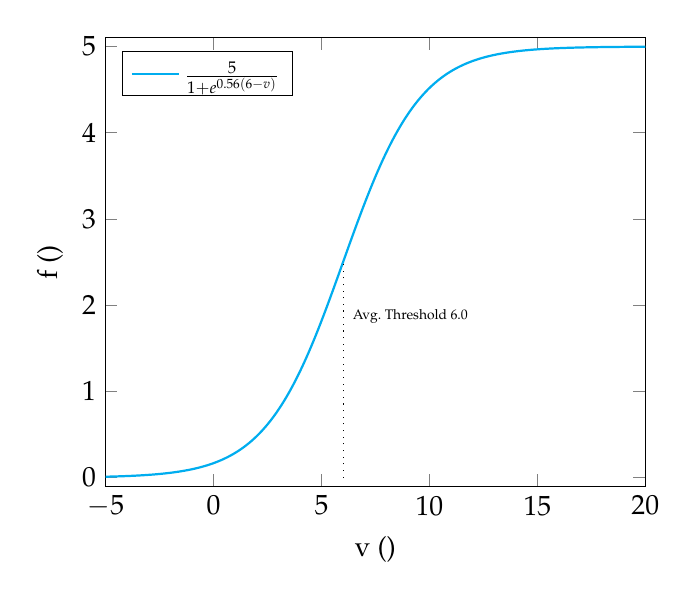
\begin{tikzpicture}
        \begin{axis}
            [
            xmin = -5, xmax = 20,
            ymin = -0.1, ymax = 5.1,
            xlabel = {v ($\SI{}{\milli\volt}$)},
            ylabel = {f ($\SI{}{\hertz}$)},
            legend pos=north west,
            legend style={nodes={scale=0.8, transform shape}},
            ],
            \addplot[
                domain = -5:20,
                samples = 200,
                smooth,
                thick,
                cyan,
            ] {5/(1+exp(0.56*(6-x)))};
            \legend{\( \frac{5}{1+e^{0.56(6-v)}} \)}
            \draw [dotted] ([xshift=0.0cm]axis cs:6,0) -- ([yshift=0.0cm]axis cs:6,2.5) node[near end,right,font=\tiny]{
                Avg.\ Threshold $\SI{6.0}{\milli\volt}$};
        \end{axis}
    \end{tikzpicture}~\caption{Sigmoid (Eq.~\ref{eq:SigmJansenRit}) \cite{jansen_neurophysiologically-based_1993}}
    \label{fig:Sigmoid}
\end{figure}

\subsubsection{PSP-Blocks}
In Physics, Linear Time-Invariant Systems (LTI systems) are oftentimes used to describe the response of
electrical circuits to arbitrary input signals.
They consist of a kernel function (or impulse-response function)
that models the system's response to a single unit-impulse.
The aforementioned PSP-Blocks are an LTI system fully represented by an impulse response function describing a PSP
relative to the onset of a pulse.
Since the PSP differs depending on the type of cell (excitatory or inhibitory),
there are two different impulse-response functions.
The parameters Jansen \& Rit used for the EPSP (Eq.~\ref{eq:ExcImpResJansenRit}) and IPSP (Eq.~\ref{eq:InhImpResJansenRit})
were based on results from van Rotterdam et al.~\cite{van_rotterdam_model_1982} and are given in Table~\ref{tab:psp_params}.
The respective plots are visualized in Fig.~\ref{fig:PSPPlot}.
%TODO: explain how the parameters can be tuned to achieve differnt results, and how that relatates to actual neurobiology
\begin{table}[H]
    \centering
    \begin{tabular}{ |c|c|c|c| }
        \hline
        \multicolumn{2}{|c|}{Parameter} & Default Value & Unit \\
        \hline
        \hline
        Exc. max. amplitude / $e$          & \(A\) & \(3.25\) & \(\SI{}{\milli\volt}\) \\
        \hline
        %TODO: EXPLAIN 'LUMPED'!!!!
        Lumped repr. of sum of exc. delays & \(a\) & \(100\)  & \(\SI{}{\hertz}\) \\
        \hline
        Inh. max. amplitude / $e$          & \(B\) & \(22\)   & \(\SI{}{\milli\volt}\) \\
        \hline
        Lumped repr. of sum of inh. delays & \(b\) & \(50\)   & \(\SI{}{\hertz}\) \\
        \hline
    \end{tabular}
    \caption{Parameters of the PSP Blocks}
    \label{tab:psp_params}
\end{table}

Excitatory impulse response:
\begin{equation}
    h_e(t) = \begin{cases}
                 Aate^{-at} & \mbox{ } t \geq 0 \\
                 0 & \mbox{ } t < 0
    \end{cases} \label{eq:ExcImpResJansenRit}
\end{equation}

Inhibitory impulse response:
\begin{equation}
    h_i(t) = \begin{cases}
                 Bbte^{-bt} & \mbox{ } t \geq 0 \\
                 0 & \mbox{ } t < 0
    \end{cases} \label{eq:InhImpResJansenRit}
\end{equation}



\begin{figure}[H]
    \centering
    \pgfplotsset{compat = newest}
    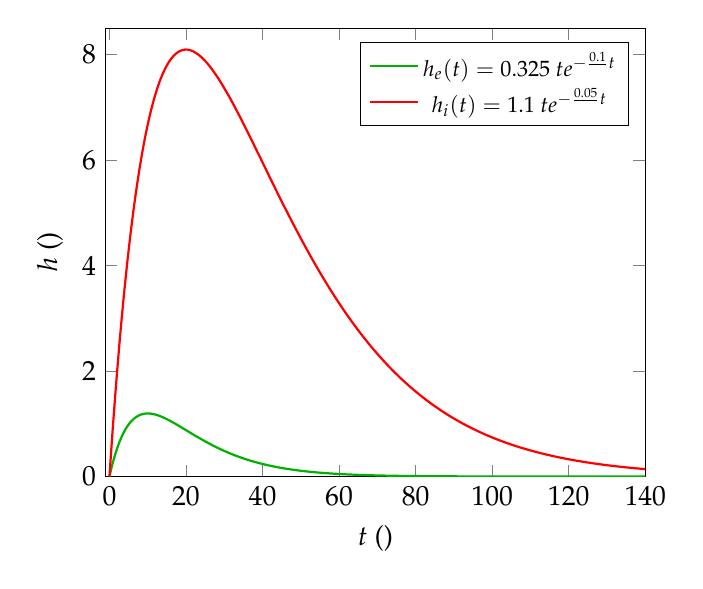
\begin{tikzpicture}
        \begin{axis}
            [
            xmin = -1, xmax = 140,
            ymin = 0, ymax = 8.5,
            xlabel = {$t$ ($\SI{}{\milli\second}$)},
            ylabel = {$h$ ($\SI{}{\milli\volt}$)},
            legend pos=north east,
            legend style={nodes={scale=0.8, transform shape}},
            ],
            \addplot[
                domain = 0:140,
                samples = 200,
                smooth,
                thick,
                green,
            ] {3.25*0.1*x*e^(-0.1*x)};
            \addplot[
                domain = 0:140,
                samples = 200,
                smooth,
                thick,
                red,
            ] {22*0.05*x*e^(-0.05*x)};

            \legend{
                $h_e(t)=0.325\frac{\SI{}{\milli\volt}}{\SI{}{\milli\second}} te^{-\frac{0.1}{\SI{}{\milli\second}}t} $,
                $ h_i(t)=1.1\frac{\SI{}{\milli\volt}}{\SI{}{\milli\second}} te^{-\frac{0.05}{\SI{}{\milli\second}}t} $
            };

        \end{axis}
    \end{tikzpicture}

    \caption{
        \textbf{Impulse Response Functions:}
        Note the small \textcolor{green}{EPSP}  (Eq.~\ref{eq:ExcImpResJansenRit}) and the
        large \textcolor{red}{IPSP}  (Eq.~\ref{eq:InhImpResJansenRit})~\parencite{jansen_neurophysiologically-based_1993}} \
    \label{fig:PSPPlot}
\end{figure}
Jansen and Rit~\cite{jansen_neurophysiologically-based_1993} justify the difference in amplitude by
referencing Lopes da Silva et al.~\cite{lopes_da_silva_models_1976} and stating that inhibitory neurons
synapse closer to the somata of pyramidal cells (often on the cell body) than excitatory cells,
increasing the effect of an inhibitory neuron about 10-fold.

The output of the Linear System defined by the PSP-Blocks is calculated by a convolution (denoted by $\ast$) of the
incoming impulse density $x(t)$ with the impulse response function $h(t)$.
For the excitatory PSP this means:\\
\begin{align}
    \overbrace{y(t)}^{\text{PSP}} = \overbrace{h_e(t)}^{\text{impulse response}} \ast \overbrace{x(t)}^{\text{impulse density}} \label{eq:convolution}
\end{align}
%%%%
% REMARK: CONVOLUTION
%%%%

\newremarkimg{Convolution}{
\begin{wrapfigure}[12]{r}{0.5\textwidth}
    \centering
    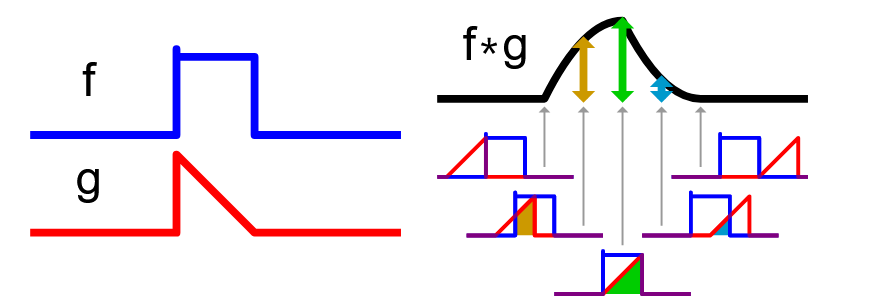
\includegraphics[width=0.45\textwidth]{Figures/convolution/wikipedia-convolution}
    \caption{\textbf{Convolution:} The area enclosed by $f(\tau)$ and $g(t-\tau)$ is the value of $(f\ast g)(t)$.\\
    \hrulefill \\
    \textit{By Cmglee - Own work, CC BY-SA 3.0  \url{https://commons.wikimedia.org/w/index.php?curid=20206883}}}
    \label{fig:Convolution}
\end{wrapfigure}
}
{
    The convolution of two functions $f(t)$ and $g(t)$ is defined as the integral of their product after one function
    has been reversed and shifted (Fig.~\ref{fig:Convolution}):
    \[f(t) \ast g(t)= \int_{-\infty}^{+\infty}f(\tau)g(t-\tau) d\tau\]
    If $f(t)$ is a unit-impulse $\delta(t)$ (in our case, this would mean that each cell of the previous population
    is firing a single action potential at the same time) the result is just $g(t)$ - a
    single full-amplitude PSP:
    \[\delta(t) \ast g(t)= \int_{-\infty}^{+\infty}\delta(\tau)g(t-\tau) d\tau = g(t)\]
    In the general case, this process can be used to mathematically model the integration of
    incoming action potential densities in the soma.\\[1em]
    Importantly, the Convolution Theorem states that the convolution of $f(t)$ and $g(t)$ becomes a
    simple multiplication when applying the Laplace Transform:
    \[\mathscr{L}\{f(t) \ast g(t)\}= \mathscr{L}\{f(t)\}\mathscr{L}\{g(t)\} = F(s)G(s)\]
    That means you can calculate a convolution with the inverse Laplace-Transform of the multiplication of
    the functions' individual Laplace-Transforms:
    \[f(t) \ast g(t)= \mathscr{L}^{-1}\{F(s)G(s)\}\]
%\end{remark}
}
Since the convolution in the time-domain is a computationally heavy operation,
it is oftentimes faster to transform the equation into the Laplace-Domain (see Eq.~\ref{eq:laplace_domain}),
apply the Convolution Theorem to perform the multiplication there,
and transform the results back to the time-domain.
This results in a second order differential equation (Eq.~\ref{eq:sec_ord_nmm}) that
can be efficiently solved by numerical integration.
To obtain this form, we need the Laplace transform $H_e(s)$ (in this context also called \textit{Transfer Function})
of our response function $h_e(t)$:
\[H_e(s) =\mathscr{L}\{h_e(t)\}  = \mathscr{L}\{Aate^{-at} \} = \frac{Aa}{(s+a)^2} = \frac{Aa}{s^2+2as+a^2}\label{eq:laplace_h_e}\]
With that, we can start to transform our initial equation (Eq.~\ref{eq:convolution}) into the desired Second Order System:
\begin{alignat}{5}
    &                                           & &&          \overbrace{y(t)}^{\text{PSP}} \quad &&=& \quad \overbrace{h_e(t)}^{\text{impulse response}} \ast \overbrace{x(t)}^{\text{impulse density}} \nonumber \\[1em]
    &                                           & \omit\rlap{applying the Laplace-Transform eliminates the convolution:}                 \nonumber \\[1em]
    &  \stackrel{\mathscr{L}}{\iff} \qquad      & &&                             Y(s) \quad &&=& \quad \overbrace{H_e(s)}^{\text{transfer function}} \cdot X(s)  \label{eq:laplace_domain} \\
    &  \iff                                     & &&                             Y(s) \quad &&=& \quad \frac{AaX(s)}{s^2+2as+a^2}  \nonumber \\
    &  \iff                                     & &&               (s^2+2as+a^2) Y(s) \quad &&=& \quad AaX(s) \nonumber \\
    &  \iff                                     & &&          s^{2}Y(s)+2asY(s)+a^{2}Y(s) \quad &&=& \quad AaX(s) \nonumber \\[1em]
    \omit\rlap{reversing the Laplace-Transform yields a differential equation in the time domain:}     \nonumber \\[1em]
    &  \stackrel{\mathscr{L}^{-1}}{\iff} \qquad & && \ddot{y}(t)+2a\dot{y}(t)+a^{2}y(t) \quad &&=& \quad Aax(t) \nonumber \\
    &  \iff                                     & &&                      \ddot{y}(t) \quad &&=& \quad Aax(t)-2a\dot{y}(t)-a^{2}y(t)  \label{eq:sec_ord_nmm} \\[1em]
    &                                           & \omit\rlap{which can be expressed as a system of two coupled first order equations:}                 \nonumber \\[1em]
    &                                           & &&                       \dot{y}(t) \quad &&=& \quad z(t)  \label{eq:y_t}\\
    &                                           & &&                       \dot{z}(t) \quad &&=& \quad Aax(t)-2az(t)-a^{2}y(t)   \label{eq:z_t}
\end{alignat}
where $y(t)$ is the resulting PSP and $x(t)$ the incoming pulse density.
This works analogously for the inhibitory case with $h_i(t)$.

\subsubsection{Full Linear System}

Taking the two first order equations for $\dot{y}(t)$ (Eq.~\ref{eq:y_t}) and $\dot{z}(t)$ (Eq.~\ref{eq:z_t})
and the Block diagram (Fig.~\ref{fig:JRBlockColored}) as a base,
we can now state the equations for the full Jansen-Rit Model with it's three populations.
Each PSP-Block $h(t)$ needs it's own system of coupled differential equations.
The value of $x(t)$ can be easily taken from the Block Diagram. $y_0(t)$ is the EPSP received by
both the EIN and IIN population, while $y_1(t)$ is the EPSP and $y_2(t)$ the IPSP received by the PC population:
\begin{equation}
    \begin{aligned}
        \dot{y}_0(t) &= z_0(t) \\
        \dot{z}_0(t) &= \fcolorbox{cyan!80}{cyan!5}{ $ Aa Sigm[y_1(t) - y_2(t)] - 2az_0(t) - a^{2}y_0(t) $}\\
        \dot{y}_1(t) &= z_1(t) \\
        \dot{z}_1(t) &= \fcolorbox{green!80}{green!5}{$ Aa(p(t) + C_{2}Sigm[C_{1}y_0(t)]) - 2az_1(t) - a^{2}y_1(t)$}\\
        \dot{y}_2(t) &= z_2(t) \\
        \dot{z}_2(t) &= \fcolorbox{red!80}{red!5}{$ Bb(C_{4}Sigm[C_{3}y_0(t)]) - 2bz_2(t) -b^{2}y_2(t)$} \\
    \end{aligned}\label{eq:jr_nmm_system}
\end{equation}

\begin{figure}[H]
    \centering
    \begin{tikzpicture}[
        pc/.style={draw=cyan!80, fill=cyan!5},
        ein/.style={draw=green!80, fill=green!5},
        iin/.style={draw=red!80, fill=red!5},
        pcLabel/.style={font=\small,text=cyan!80},
        einLabel/.style={font=\small,text=green!80},
        iinLabel/.style={font=\small,text=red!80},
        rectNode/.style={draw=black!80, thick},
        roundNode/.style={circle, draw=black!80, thick},
        ]
	    \input{Chapters/Chapter_02_Technical_Concepts/tikz/jr_simple_block_tikz}
\end{tikzpicture}
    \caption{Colored Block diagram, visualizing the components of (Eq.~\ref{eq:jr_nmm_system})}
    \label{fig:JRBlockColored}
\end{figure}

\subsubsection{Model Input}

The model input $p(t)$ represents the average activity of populations outside the modeled
column that synapse on the columns PC population.
Since this activity's source is so diverse, it is modeled by white noise ($120-\SI{320}{\hertz}$).

%\begin{wrapfigure}[5]{r}{0.32\textwidth}
\begin{figure}[H]
    \centering
    \pgfplotsset{compat = newest}
    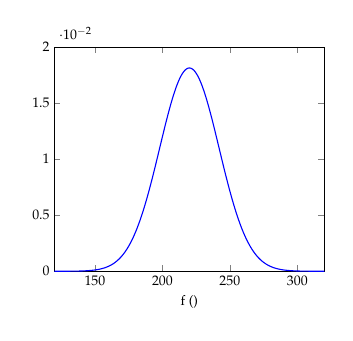
\begin{tikzpicture}[scale=0.5]
        \begin{axis}
            [
            xmin = 120, xmax = 320,
            ymin = 0, ymax = 0.02,
            xlabel = {f ($\SI{}{\hertz}$)},
            legend pos=outer north east,
            legend style={nodes={scale=1.2, transform shape}},
            ],
            \addplot[
                domain = 120:320,
                samples = 200,
                smooth,
                thick,
                blue,
            ]{(exp(-0.5*((x-220)/22)^2))/(22*sqrt(2*pi))};
            %\legend{$\frac{1}{22\sqrt{2\pi}}e^{-\frac{1}{2}(\frac{x-220}{22})^2}$};

        \end{axis}
    \end{tikzpicture}

    \caption{
        \textbf{Input distribution.}
        The input frequency representing $p(t)$ is sampled from a normal distribution with $\mu=220$ and $\sigma=22$}
    \label{fig:ModelInput}
        %\end{wrapfigure}
\end{figure}

\subsubsection{Connectivity Constants}\label{subsubsec:connectivity_constants}

A sensible choice for the Connectivity Constants $C_1$ to $C_4$ was determined by Jansen and Rit empirically by
defining a histologically motivated relationship between them ($C = C_1 = \frac{C_2}{0.8} = \frac{C_3}{0.25} =
\frac{C_4}{0.25}$) and varying $C$ until the system produced the desired natural alpha-like activity at $C=C_1=135
\Rightarrow C_2=108; C_3=C_4=33.75$.
Varying $C$ can account for common synaptic phenomena like
neurotransmitter depletion~\parencite{jansen_electroencephalogram_1995}.


\subsubsection{Model Output}
Simulated data from $y_1-y_2$ while varying $C$ is plotted in Fig.~\ref{fig:jr_c_sweep},
which is perfectly reproducing ~\cite[Fig. 3]{jansen_electroencephalogram_1995}.
The desired alpha-activity is clearly visible for $C = 135$,
which led Jansen \& Rit to their choice of default parameters mentioned in Sec.~\ref{subsubsec:connectivity_constants}.
The other plots give an insight into the models capabilities of producing varying forms of activity,
but in this work we will not further explore variations of $C$.
An interesting phenomenon is, however,
that very low and very high connectivity both leads to the system being entirely noise-driven,
which produces signals with identical form, but different amplitude for different values of $C$ (compare $C=1350$ and $C=68$),
as long as they are supplied with identical input.
All signals in Fig.~\ref{fig:jr_c_sweep} were generated with the same pre-sampled random input.

Fig.~\ref{fig:jr_psd} shows the Power Spectral Density (PSD) of the chosen signal and the corresponding spectrogram for a
60 second simulation session is given in Fig.~\ref{fig:jr_spec}.
It is clearly visible that the signal is mainly composed of a single sinusoidal component at  $\approx \SI{11}{\hertz}$.
\begin{figure}[H]
    \centering
    \subfloat[\textbf{JR Model Output for varying $C$.} \\
    Well defined alpha-activity is visible at $C=135$.\\
    ]{\label{fig:jr_c_sweep}
        \resizebox{!}{10cm}{
            \begin{tikzpicture}
                \pgfplotsset{
                %% Axis
                    scale only axis,
                    width=0.8\linewidth,
                    height=2cm,
                    every axis/.append style={
                        line width=1pt,
                        tick style={line width=0.8pt},
                        %   grid style={dashed, black!20},
                        %  grid=major,
                    },
        %               %% X-Axis
                    xmin=1.0,
                    xmax=3,
                }
                \begin{groupplot}
                    [
                    group style={
                        group size=1 by 6,
                        vertical sep=2mm,
                        xlabels at=edge bottom,
                        xticklabels at=edge bottom,
                    },
                    yticklabel style={
                        /pgf/number format/fixed,
                        /pgf/number format/precision=2
                    },
                    legend style={nodes={scale=0.8, transform shape}, thin},
                    legend image post style={scale=0},
                    xlabel=$t (\SI{}{\second})$
                    ]
        %           \pgfplotsinvokeforeach{0,1,2,3,4,5}{
        %             \nextgroupplot
        %             \addplot [line width=1pt,solid,color=cyan] table[x=x,y= c#1 ,col sep=comma]{data/test135.csv};
        %          }
                    \nextgroupplot
                    \addplot [line width=1pt,solid] table[x=x,y=c0 ,col sep=comma]{data/simple_c_sweep.csv};
                    \legend{$C=68$};
                    \nextgroupplot
                    \addplot [line width=1pt,solid] table[x=x,y=c1 ,col sep=comma]{data/simple_c_sweep.csv};
                    \legend{$C=128$};
                    \nextgroupplot
                    \addplot [line width=1pt,solid] table[x=x,y=c2 ,col sep=comma]{data/simple_c_sweep.csv};
                    \legend{$C=135$};
                    \nextgroupplot[ylabel=v ($\SI{}{\micro\volt}$), every axis y label/.append style={at=(ticklabel cs:1.0)}]
                    \addplot [line width=1pt,solid] table[x=x,y=c3 ,col sep=comma]{data/simple_c_sweep.csv};
                    \legend{$C=270$};
                    \nextgroupplot
                    \addplot [line width=1pt,solid] table[x=x,y=c4 ,col sep=comma]{data/simple_c_sweep.csv};
                    \legend{$C=675$};
                    \nextgroupplot
                    \addplot [line width=1pt,solid] table[x=x,y=c5 ,col sep=comma]{data/simple_c_sweep.csv};
                    \legend{$C=1350$};

                \end{groupplot}
            \end{tikzpicture}
        }
    }
    \hfill
    \subfloat[\textbf{PSD of JR Model Output.} \\
                     ($C=135$, Multitapered)]{\label{fig:jr_psd}
        \resizebox{7cm}{5.3cm}{
            \pgfplotsset{compat = newest}
            \begin{tikzpicture}[scale=0.5]
                \begin{axis}
                    [ylabel=$\SI{}{\volt/\hertz}$
                    ],
                    \addplot [line width=.5pt,solid, cyan]
                        table[x=x,y=y ,col sep=comma]{data/methodology/psd_multitaper_jr.csv};

                \end{axis}
            \end{tikzpicture}

        }
    }
    \subfloat[\textbf{Spectrogram of JR Model Output.} \\
                     ($C=135$)]{\label{fig:jr_spec}
        \resizebox{7.5cm}{!}{
            \import{data/rest_sim}{JR_REST_60.pgf}
        }
    }
    %\hfill
    \caption{\textbf{Properties of JR Model Output}}
    \label{fig:jr_model_out_props}
\end{figure}

\pagebreak

\subsection{The Sub-Population-Extension by David and Friston}\label{subsec:the-david-and-friston-model}
While the JR model succeeds in generating realistic alpha activity,
real EEG Signals contain much richer spectra~\parencite{steriade_impact_2001}.
David and Friston~\cite{david_neural_2003} proposed a modification to the JR model,
that could produce a more realistic frequency spectrum by adding sub-populations to the model.
They can be tuned individually to produce oscillations in different frequencies.

\subsubsection{Introducing sub-populations}

David and Friston slightly redefine the impulse response function $h(t)$ (Eq.~\ref{eq:ExcImpResJansenRit})
in the PSP-Blocks by introducing the parameters $H$ and $\tau$ (see Table~\ref{tab:davidfriston}),
which are just a minor alteration of $A$ and $a$.
\[ h(t)=Aate^{-at} => h(t)=\frac{H}{\tau}te^{-\frac{1}{\tau}} \]
Before tweaking these parameters to produce slower or faster kinetics,
they define the products $H_e\tau_e=\SI{0.0325}{\milli\volt\second}$ and $H_i\tau_i=\SI{0.44}{\milli\volt\second}$ as constants.
This is done to preserve the oscillatory behavior of each population~\parencite{david_neural_2003}.
When varying $\tau$, $H$ is therefore adjusted
accordingly ($H_e=\frac{\SI{0.0325}{\milli\volt\second}}{\tau_e}$, $H_i=\frac{\SI{0.44}{\milli\volt\second}}{\tau_i}$).
\begin{table}[H]
    \centering
    \begin{tabular}{ |c|c|c|c|c| }
        \hline
        \multicolumn{2}{|c|}{Parameter} & Value & Unit & Relation to \parencite{jansen_electroencephalogram_1995} \\
        \hline
        \hline
        \rule{0pt}{3ex}Excitatory delays        & \(\tau_e\) & \(10\) & $\SI{}{\milli\second}$  & $ \tau_e = \frac{1}{a} $ \\[1.2ex]
        \hline
        \rule{0pt}{3ex}Inhibitory delays        & \(\tau_i\) & \(20\) & $\SI{}{\milli\second}$  & $ \tau_i = \frac{1}{b} $\\[1.2ex]
        \hline
        \rule{0pt}{3ex}Excitatory synaptic gain & \(H_e\)    & \(3.25\) & $\SI{}{\milli\volt}$ & $ H_e = A $ \\[1.2ex]
        \hline
        \rule{0pt}{3ex}Inhibitory synaptic gain & \(H_i\)    & \(22\)   & $\SI{}{\milli\volt}$ & $ H_i = B $ \\[1.2ex]
        \hline
    \end{tabular}
    \caption{Parameters of the PSP Blocks after David \& Friston~\cite{david_neural_2003}}
    \label{tab:davidfriston}
\end{table}
\fcolorbox{red}{red!10}{\parbox{\textwidth}{
    \textbf{Attention:} For the remainder of this work, the indices $[0,\dots,N]$ for $y$, $h$, $\tau$ and $H$ refer only to
    the subpopulations within a single population.
    The indices used above in the formulation for the Simple Jansen-Rit Model (and the Block Diagram) should not
    be confused with these.
    However, $e$ and $i$ as indices still denote excitatory and inhibitory populations respectively.}} \\[1em]

\noindent
To introduce subpopulations, they split up the general impulse response function $h(t)$ in $N$ individual
sub-functions:
\[h_n(t) = \frac{H_n}{\tau_n}te^{-\frac{1}{\tau_n}}\]\\
\noindent
The previously defined general PSP-Block Equation:
\[y(t)=h(t)\ast x(t)\]
then becomes:
\[y(t)=\sum_{n=0}^{N}{(w_n \cdot h_n(t) \ast x(t))} \hspace{2em}
\text{with}
\hspace{2em} \sum_{n=0}^{N}w_n = 1 \hspace{2em}
\text{and}
\hspace{2em} 0 \leq w_n \leq 1\]
with N individually weighted ($w_n$) and parameterized ($h_n(t)$) subpopulations. \\
We can then declare:
\[y_n(t) = h_n(t) \ast x(t) \quad \text{and} \quad y(t) = \sum_{n=0}^{N} (w_{n}y_n)\]
which produces the following differential equations for a single PSP Block:

\begin{equation}
    \begin{aligned}
        \dot{y}_0(t) &= z_0(t) \\
        \dot{z}_0(t) &= \frac{H_0}{\tau_0} x(t) - \frac{2}{\tau_0}z_0(t) - \left(\frac{1}{\tau_0}\right)^{2}y_0(t)\\
        &\dots\\
        \dot{y}_N(t) &= z_N(t) \\
        \dot{z}_N(t) &= \frac{H_N}{\tau_N} x(t) - \frac{2}{\tau_N}z_N(t) - \left(\frac{1}{\tau_N}\right)^{2}y_N(t)\\
        y(t)         &= w_{0}y_0 + \dots + w_{N}y_N\\
    \end{aligned}\label{eq:davidfriston_subpops}
\end{equation}

\begin{figure}[H]
    \begin{tikzpicture}
	\node(sout){};
	\node[shape=rectangle, draw=black, left=0.3cm of sout.center] (SigmPC) {$x(t)$};
	
	\node[shape=rectangle, draw=black, above right=1cm and 2.5cm of sout.center] (H1) {$h_{e_0}(t)$};
	\node[shape=rectangle, draw=black, fill=white, below right=0.2cm and 0.2cm of H1.west] (H2) {$h_{e_1}(t)$};
	\node[shape=rectangle, draw=black, fill=white, below right=2cm and 0.8cm of H2.west] (HN) {$h_{e_N}(t)$};
	\draw[black!80, linedots, linedot diameter=4pt, linedot spacing=25pt, shorten <=8pt, shorten >=8pt] (H2.south) --
    (HN.north);
	\node[shape=rectangle, dotted, draw=black, fill=white, fill opacity=0.7, text opacity=1, below right=0.8cm and 0.4cm of H2.west] (Hen) {$h_{e_n}(t)$};
	
	
	\node[left=0.3cm of H1.west](x1){};
	\node[left=0.45cm of H2.west](x2){};
	\node[left=0.85cm of Hen.west](xen){};
	\node[left=1.3cm of HN.west](xN){};
	
	\node[shape=circle, draw=black, right=2cm of H1] (w1) {\small$w_0$};
	\node[shape=circle, draw=black,fill=white, right=2cm of H2] (w2) {\small$w_1$};
	\node[shape=circle, dotted, draw=black, right=2cm of Hen] (wen) {\small$w_n$};
	\node[shape=circle, draw=black, right=2cm of HN] (wN) {\small$w_N$};
	
	
	\node[right=1.1cm of w1.east](y1){};
	\node[right=0.9cm of w2.east](y2){};
	\node[right=0.5cm of wen.east](yen){};
	\node[right=0.001cm of wN.east](yN){};
	
	\node[shape=rectangle, draw=black, right=10cm of sout.center] (pout){$y(t)$};
	
	
	\draw[-] (SigmPC.east) -- (sout.center);
	
	\draw[-] (sout.center) .. controls +(3:1.2) and +(10:-1.5) .. (x1.center);
	\draw[-] (sout.center) .. controls +(3:1.2) and +(10:-1.5) .. (x2.center);
	\draw[-, dotted] (sout.center) .. controls +(3:1.2) and +(10:-1.5) .. (xen.center);
	\draw[-] (sout.center) .. controls +(3:1.2) and +(10:-1.5) .. (xN.center);
	
	
	\draw[->] (x1.center) |- (H1.west);
	\draw[->] (x2.center) |- (H2.west);
	\draw[->, dotted] (xen.center) |- (Hen.west);
	\draw[->] (xN.center) |- (HN.west);
	
	\draw[->] (H1.east) -- (w1.west) node [above, midway]{\tiny$y_0(t)$};
	\draw[->] (H2.east) -- (w2.west)node [above, midway]{\tiny$y_1(t)$};
	\draw[->, dotted] (Hen.east) -- (wen.west)node [above, midway]{\tiny$y_n(t)$};
	\draw[->] (HN.east) -- (wN.west)node [above, midway]{\tiny$y_N(t)$};
	
	
	
	\draw[-] (w1.east) |- (y1.center);
	\draw[-] (w2.east) |- (y2.center);
	\draw[-, dotted] (wen.east) |- (yen.center);
	\draw[-] (wN.east) |- (yN.center);
	
	\draw[->, very thin] (y1.center) .. controls +(3:1.2) and +(10:-1.5) .. (pout.west);
	\draw[->, very thin] (y2.center) .. controls +(3:1.2) and +(10:-1.5) .. (pout.west);
	\draw[->, dotted, thin] (yen.center) .. controls +(3:1.2) and +(10:-1.5) .. (pout.west);
	\draw[->, very thin] (yN.center) .. controls +(3:1.2) and +(10:-1.5) .. (pout.west);
	
\end{tikzpicture}
    \caption{Example of subpopulations ($h_{e_0}(t), \dots, h_{e_N}(t)$) forming an excitatory population $h_e(t)$}
    \label{fig:exc_subpops}
\end{figure}

\vspace{1em}
\noindent
David and Friston further propose an example with two subpopulations for each population.
The parameters are listed in Fig.~\ref{fig:PSPPlotDavidFriston}.
While the kinetics for the first subpopulation ($\tau_{e_0}, \tau_{i_0}$) in each population are still close
to those of the original populations ($\tau_e=10ms, \tau_i=20ms$, which produce alpha activity),
each of the second subpopulation's  ($\tau_{e_1}, \tau_{i_1}$) parameters were chosen to produce gamma activity.
The associated weights are  $w_0=0.8$ and $w_1=0.2$ for both populations,
favouring the original slower kinetics,
as this combination results in the most realistic frequency distribution according to the authors (compare Fig.~\ref{fig:df_psd}).

\begin{figure}[H]
    \centering
    \pgfplotsset{compat = newest}
    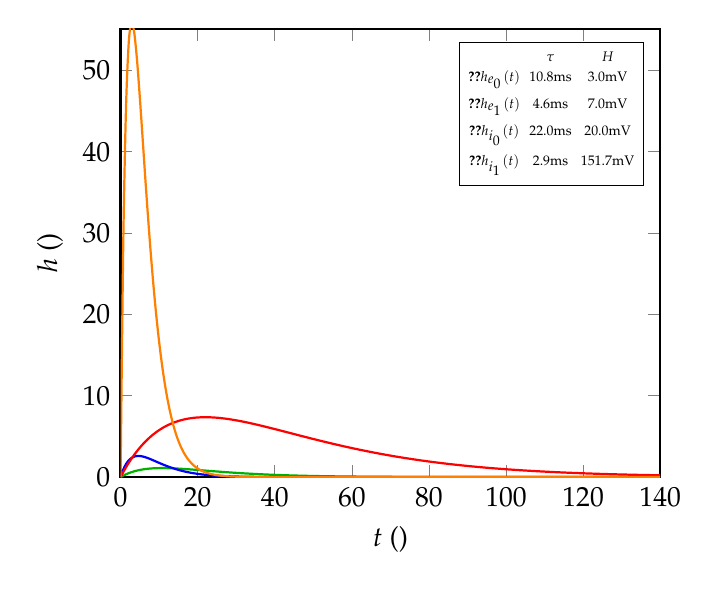
\begin{tikzpicture}
        \begin{axis}
            [
            xmin = 0, xmax = 140,
            ymin = 0, ymax = 55.1,
            xlabel = {$t$ ($\SI{}{\milli\second}$)},
            ylabel = {$h$ ($\SI{}{\milli\volt}$)},
            legend pos=north east,
            legend style={nodes={scale=0.8, transform shape}},
            domain = 0:140,
            samples = 200,
            smooth,
            thick,
            ],
            \addplot[green] {(3.01/10.8)*x*e^(-(1/10.8)*x)};\label{plot:line1}
            \addplot[blue] {(7.07/4.6)*x*e^(-(1/4.6)*x)};\label{plot:line2}
            \addplot[red] {(20/22)*x*e^(-(1/22)*x)};\label{plot:line3}
            \addplot[orange] {(151.72/2.9)*x*e^(-(1/2.9)*x)};\label{plot:line4}
            \coordinate (legend) at (axis description cs:0.97,0.97);
        \end{axis}
        \tiny
        \matrix [
            draw,
            matrix of nodes,
            anchor=north east,
        ] at (legend) {

            & $\tau$ &    $H$  \\
            \ref{plot:line1}$h_{e_0}(t)$ & 10.8ms &   3.0mV \\
            \ref{plot:line2}$h_{e_1}(t)$ &  4.6ms &   7.0mV \\
            \ref{plot:line3}$h_{i_0}(t)$ & 22.0ms &  20.0mV \\
            \ref{plot:line4}$h_{i_1}(t)$ &  2.9ms & 151.7mV \\
        };
    \end{tikzpicture}

    \caption{\textbf{PSP functions for subpopulations as proposed by David \& Friston~\cite{david_neural_2003}:} \\
        The subpopulations $h_{e_1}$ and $h_{i_1}$ are faster
        than the original populations and their slower variations in $h_{e_0}$ and $h_{i_0}$ and
        elicit activity with higher frequencies.
    }
    \label{fig:PSPPlotDavidFriston}
\end{figure}

\subsubsection{Model Output}
The values chosen by David \& Friston indeed produce a frequency distribution
with a broad distribution over the alpha and beta bands (Fig.~\ref{fig:df_psd}).
On average, the frequencies peak in alpha ($~\SI{12}{\hertz}$), as visible in the PSD plot,
however, the spectrogram (Fig.~\ref{fig:df_spec}) reveals fluctuations of the peak frequency
between the alpha and beta band over time.
The average frequency amplitude is harshly reduced compared to the JR model,
which becomes clear when scaling the JR model's PSD (Fig.~\ref{fig:jr_psd_rescaled})
and spectrogram (Fig.~\ref{fig:jr_spec_rescaled}) to the same value ranges.

\begin{figure}[H]
    \centering
    \subfloat[\textbf{PSD of DF Model Output.} (Multitapered)]{\label{fig:df_psd}
        \resizebox{7cm}{5.3cm}{
            \pgfplotsset{compat = newest}
            \begin{tikzpicture}[scale=0.5]
                \begin{axis}
                    [ymax=0.000000003
                    ],
                    \addplot [line width=.5pt,solid, cyan]
                        table[x=x,y=y ,col sep=comma]{data/methodology/psd_multitaper_df_35.csv};

                \end{axis}
            \end{tikzpicture}
        }
    }
    \subfloat[\textbf{Spectrogram of DF Model Output.}]{\label{fig:df_spec}
        \resizebox{7.5cm}{!}{
            \import{data/rest_sim}{DF_REST_60.pgf}
        }
    }
    \hfill
    \subfloat[\textbf{PSD of JR Model Output.} \\
              (see Fig.~\ref{fig:jr_psd})\\
              Scaled to match intensity for comparison]{\label{fig:jr_psd_rescaled}
        \resizebox{7cm}{5.3cm}{
            \pgfplotsset{compat = newest}
            \begin{tikzpicture}[scale=0.5]
                \begin{axis}
                    [ymax=0.000000003
                    ],
                    \addplot [line width=.5pt,solid, cyan]
                        table[x=x,y=y ,col sep=comma]{data/methodology/psd_multitaper_jr.csv};

                \end{axis}
            \end{tikzpicture}
        }
    }
    \subfloat[\textbf{Spectrogram of JR Model Output.}\\
              (see Fig.~\ref{fig:jr_spec})\\
              Scaled to match intensity for comparison]{\label{fig:jr_spec_rescaled}
        \resizebox{7.5cm}{!}{
            \import{data/rest_sim}{JR_REST_60_dfscale.pgf}
        }
    }
    \caption{\textbf{Properties of DF Model Output in comparison to JR model}}
    \label{fig:df_model_out_props}
\end{figure}
\pagebreak
%

%----------------------------------------------------------------------------------------
%	UNDERSTANDING THE PSP BLOCK DIFFERENTIAL EQUATIONS
%----------------------------------------------------------------------------------------
\pagebreak
.
\pagebreak
\section{comparision of psp blocks}


\subsection{\parencite{wilson_excitatory_1972}}

\begin{table}[H]
	\centering
	\begin{tabular}{ |c|c|c|c| } 
		\hline
		\multicolumn{2}{|c|}{Parameter}  & Sensible Value & Unit \\
		\hline
		\hline
		prop. of exc. cells firing at $t$ & \(E(t)\) & \( \) & \( \) \\
		\hline
		prop. of inh. cells firing at $t$ & \(I(t)\) & \( \) & \( \) \\
		\hline
		absolute refractory period & $r$ & 4 & $ms$ \\
		\hline
		firing threshold & $\theta$ & & $mV$ \\
		\hline
		propagation delay & $\tau$ & 10 & $ms$ \\
		\hline
		stimulation decay & $\alpha$ & & $mV/s$ (?) \\
		\hline
	\end{tabular}
	\caption{Parameters of \parencite{wilson_excitatory_1972}}
	\label{table:params_wilsoncowan}
\end{table}

Proportion of cells that are excitable at $t$:
\begin{equation}
	1 - \underbrace{\int_{t-r}^{t} E(t') dt'}_{\text{refractory cells}}
\end{equation}

Subpopulation response function (Sigmoid):
\begin{equation}
	\mathscr{S}(x) = \int_{0}^{x(t)} D(\theta) d\theta 
\end{equation}

Excitation in exc. cell
\begin{equation}
	E(t+\tau) = \overbrace{(1 - \underbrace{\int_{t-r}^{t} E(t') dt'}_{\text{refractory cells}}}^{\text{excitable cells}}) \cdot \mathscr{S}_e \cdot \int_{-\infty}^{t}\alpha(t-t') \cdot [C_1E(t') - C_2(I(t') + P(t')] dt'
\end{equation}


\subsection{\parencite{zetterberg_performance_1978} (referencing a model developed in 1973)}

\subsection{\parencite{lopes_da_silva_model_1974}}



\subsection{\parencite{jansen_electroencephalogram_1995}}


\begin{table}[H]
	\centering
	\begin{tabular}{ |c|c|c|c| } 
		\hline
		\multicolumn{2}{|c|}{Parameter}  & Default Value & Unit \\
		\hline
		\hline
		Excitatory synaptic gain & \(A\) & \(3.25\) & \(mV\) \\
		\hline
		Lumped repr. of sum of exc. delays & \(a\) & \(100\) & \(Hz\) \\
		\hline
		Inhibitory synaptic gain & \(B\) & \(22\) & \(mV\) \\
		\hline
		Lumped repr. of sum of inh. delays & \(b\) & \(50\) & \(Hz\) \\
		\hline
	\end{tabular}
	\caption{Parameters of the PSP Blocks2}
	\label{table:psp_params2}
\end{table}

The differential equations for the Second Order System  of this model can be derived by transformations in the Laplace-Domain (see \ref{eq:laplace_domain2}). To obtain the required Transfer-Function, we need the Laplace transform $H_e(s)$ of our response function $h_e(t)$. This is shown in \ref{eq:laplace_h_e2}.


\begin{equation}
	H_e(s) =\mathscr{L}\{h_e(t)\}  = \mathscr{L}\{Aate^{-at} \} = \frac{Aa}{(s+a)^2} = \frac{Aa}{s^2+2as+a^2}\label{eq:laplace_h_e2}
\end{equation}



\begin{alignat}{5}
	&                                           & &&          \overbrace{Y(s)}^{\text{output}} \quad &&=& \quad \overbrace{H_e(s)}^{\text{transfer function}} \overbrace{X(s)}^{\text{input}} \label{eq:laplace_domain2} \\
	&  \iff                                     & &&                             Y(s) \quad &&=& \quad \frac{Aa}{s^2+2as+a^2} X(s) \nonumber \\ 
	&  \iff                                     & &&               (s^2+2as+a^2) Y(s) \quad &&=& \quad AaX(s) \nonumber \\ 
	&  \iff                                     & &&          s^2Y(s)+2asY(s)+a^2Y(s) \quad &&=& \quad AaX(s) \nonumber \\ 
	&  \stackrel{\mathscr{L}^{-1}}{\iff} \qquad & && \ddot{y}(t)+2a\dot{y}(t)+a^2y(t) \quad &&=& \quad Aax(t) \nonumber \\ 
	&  \iff                                     & &&                      \ddot{y}(t) \quad &&=& \quad Aax(t)-2a\dot{y}(t)-a^2y(t)  \label{eq:sec_ord_nmm2} \\[1em]
	&                                           & \omit\rlap{which can be expressed as two first order equations:}                 \nonumber \\[1em]
	&                                           & &&                       \dot{y}(t) \quad &&=& \quad z(t) \nonumber \\ 
	&                                           & &&                       \dot{z}(t) \quad &&=& \quad Aax(t)-2az(t)-a^2y(t) \nonumber 
\end{alignat}

Comparing (\ref{eq:sec_ord_nmm2}) to the General Form of Second Order Systems (\ref{eq:gen_sec_order_sys2}), we can see that this is a critically damped system ($\zeta = 1$) and the natural frequency $\tau$ of the system is set at $a$.

\begin{align}
	f(t) &= \ddot{y}(t)+ 2\zeta \tau\dot{y}(t) + \tau^2y(t) \nonumber \\ 
	\iff  \ddot{y}(t) &= f(t) - 2\zeta \tau\dot{y}(t) - \tau^2y(t)  \label{eq:gen_sec_order_sys2}
\end{align}

\begin{figure}[H]
	\centering
	\includegraphics[width=12cm]{Figures/jansenrit/jansen_rit_ode_graph.png}
	\caption{Simplified Model after \parencite{jansen_electroencephalogram_1995}}
	\label{Fig: Jansen Rit Simple2}
\end{figure}

Taking the two equations for $\dot{y}$ and $\dot{z}$ as a base, we can now state the equations for the full NMM with it's three populations:

\begin{equation}
	\begin{aligned}
		\dot{y}_0(t) &= y_3(t) \\
		\dot{y}_3(t) &= \fcolorbox{green}{white!30}{$ Aa Sigm[y_1(t) - y_2(t)] - 2ay_3(t) - a^2y_0(t) $}\\
		\dot{y}_1(t) &= y_4(t) \\
		\dot{y}_4(t) &= \fcolorbox{red}{white!30}{$ Aa(p(t) + C_2Sigm[C_1y_0(t)]) - 2ay_4(t) - a^2y_1(t)$}\\
		\dot{y}_2(t) &= y_5(t) \\
		\dot{y}_5(t) &= \fcolorbox{blue}{white!30}{$ Bb(C_4Sigm[C_3y_0(t)]) - 2by_5(t) -b^2y_2(t)$} \\
	\end{aligned}
\end{equation}

\begin{equation}
	\begin{aligned}
		\frac{d}{dt}PSP_{EIN} &= PSP_{t_{EIN}} \\
		\frac{d}{dt}PSP_{t_{EIN}} &= \fcolorbox{lime}{white!30}{$ \frac{h_e}{\tau_e}\cdot C_1 Sigm[PSP_{PC}]  -\frac{2}{\tau_e} \cdot PSP_{t_{EIN}} - \left(\frac{1}{\tau_e}\right)^2 \cdot PSP_{EIN} $}\\
		\frac{d}{dt}PSP_{IIN} &= PSP_{t_{IIN}} \\
		\frac{d}{dt}PSP_{t_{IIN}} &= \fcolorbox{teal}{white!30}{$ \frac{h_e}{\tau_e} \cdot C_3 Sigm[PSP_{PC}]  -\frac{2}{\tau_e} \cdot PSP_{t_{IIN}} - \left(\frac{1}{\tau_e}\right)^2 \cdot PSP_{IIN} $}\\
		\frac{d}{dt}PSP_{PCE} &= PSP_{t_{PCE}} \\
		\frac{d}{dt}PSP_{t_{PCE}} &= \fcolorbox{red}{white!30}{$ \frac{h_e}{\tau_e} \cdot (u + C_2 Sigm[PSP_{EIN}])  -\frac{2}{\tau_e} \cdot PSP_{t_{PCE}} - \left(\frac{1}{\tau_e}\right)^2 \cdot PSP_{PCE} $}\\
		\frac{d}{dt}PSP_{PCI} &= PSP_{t_{PCI}} \\
		\frac{d}{dt}PSP_{t_{PCI}} &= \fcolorbox{blue}{white!30}{$ \frac{h_i}{\tau_i} \cdot C_4 Sigm[PSP_{IIN}])  -\frac{2}{\tau_i} \cdot PSP_{t_{PCI}} - \left(\frac{1}{\tau_i}\right)^2 \cdot PSP_{PCI} $}\\
		PSP_{PC} &= PSP_{PCE} - PSP_{PCI}\\
	\end{aligned}
\end{equation}    

\begin{figure}[H]
	\centering
	\includegraphics[width=12cm]{Figures/jansenrit/pyrates_ode_graph.png}
	\caption{Jansen-Rit Model with Modules in PyRates \parencite{gast_pyratespython_2019}}
	\label{Fig: PyratesODE}
\end{figure}

\subsection{\parencite{gast_pyratespython_2019}}
\begin{table}[H]
	\centering
	\begin{tabular}{ |c|c|c|c|c| } 
		\hline
		\multicolumn{2}{|c|}{Parameter}  & Value & Unit & Relation to \parencite{jansen_electroencephalogram_1995} \\
		\hline
		\hline
		\rule{0pt}{3ex}Excitatory delays & \(\tau_e\) & \(0.01\) & $s$ & $ a = \frac{1}{\tau_e} $ \\[1.2ex]
		\hline
		\rule{0pt}{3ex}Inhibitory delays & \(\tau_i\) & \(0.02\) & $s$ & $ b = \frac{1}{\tau_i} $\\[1.2ex]
		\hline
		\rule{0pt}{3ex}Excitatory synaptic gain & \(h_e\) & \(3.25\) & $mV$ & $ A = h_e $ \\[1.2ex]
		\hline
		\rule{0pt}{3ex}Inhibitory synaptic gain & \(h_i\) & \(22\) & $mV$ & $ B = h_i $ \\[1.2ex]
		\hline
		\rule{0pt}{3ex}PSP of $pop$ & \(PSP_{pop}\) &  & & $ PSP_{pop} = y  $ \\[1.2ex]
		\hline
		\rule{0pt}{3ex} Deriv. of PSP of $pop$  & \(PSP_{t_{pop}}\) &  & & $\frac{d}{dt}PSP_{pop} = PSP_{t_{pop}} = z = \dot{y}$ \\[1.2ex]
		\hline
	\end{tabular}
	\caption{Parameters of the PyRates ODEs}
\end{table}


$y_0 = PSP_{PC}, y_1 ~= PSP_{PCE}, y_2 ~= PSP_{PCI}, y_3=?$ 

\begin{equation}
	\begin{aligned}
		\frac{d}{dt}PSP_{EIN} &= PSP_{t_{EIN}} \\
		\frac{d}{dt}PSP_{t_{EIN}} &= \frac{h_e}{\tau_e}\cdot C_1 Sigm[PSP_{PC}]  -\frac{2}{\tau_e} \cdot PSP_{t_{EIN}} - \left(\frac{1}{\tau_e}\right)^2 \cdot PSP_{EIN} \\
		\frac{d}{dt}PSP_{IIN} &= PSP_{t_{IIN}} \\
		\frac{d}{dt}PSP_{t_{IIN}} &= \frac{h_e}{\tau_e} \cdot C_3 Sigm[PSP_{PC}]  -\frac{2}{\tau_e} \cdot PSP_{t_{IIN}} - \left(\frac{1}{\tau_e}\right)^2 \cdot PSP_{IIN}\\
		\frac{d}{dt}PSP_{PCE} &= PSP_{t_{PCE}} \\
		\frac{d}{dt}PSP_{t_{PCE}} &= \fcolorbox{green}{white!30}{$ \frac{h_e}{\tau_e} \cdot (u + C_2 Sigm[PSP_{EIN}])  -\frac{2}{\tau_e} \cdot PSP_{t_{PCE}} - \left(\frac{1}{\tau_e}\right)^2 \cdot PSP_{PCE} $}\\
		\frac{d}{dt}PSP_{PCI} &= PSP_{t_{PCI}} \\
		\frac{d}{dt}PSP_{t_{PCI}} &= \fcolorbox{red}{white!30}{$ \frac{h_i}{\tau_i} \cdot C_4 Sigm[PSP_{IIN}])  -\frac{2}{\tau_i} \cdot PSP_{t_{PCI}} - \left(\frac{1}{\tau_i}\right)^2 \cdot PSP_{PCI} $}\\
		PSP_{PC} &= PSP_{PCE} - PSP_{PCI}\\
	\end{aligned}
\end{equation}                        



\pagebreak
%----------------------------------------------------------------------------------------
%	SECTION 1
%----------------------------------------------------------------------------------------


\section{[TEMP] Neural Mass Models}

Neural Mass Models are computational models of neural populations that aim to simulate population dynamics instead of individual neurons. They operate on the assumption that some of the most studied [frequency-based/state] effects can be modelled by treating a neural population as a single computational unit with one input and one output, representing the sum of all enclosed neuronal activity, thus greatly reducing the computational cost of the model. By combining just a few different populations in a biologically motivated structure, these models can indeed reproduce signals with realistic components. However, when using a model with this degree of simplification, one must always be aware of it's limitations. [citation-needed]

\subsection{History}

\begin{itemize}
	\item \parencite{wilson_excitatory_1972}
	\begin{itemize}
		\item Model for stuff
		\item \( x^n + y^n = z^n \cdot \sqrt{15x} \)
	\end{itemize}
	\item \parencite{lopes_da_silva_model_1974}
	\begin{itemize}
		\item Model for Alpha Activity Generation based on empirically collected physiological parameters 
		\item Histological data of thalamo-cortical relay cells (TCR) and interneurons (IN)
		\item postulated concept: TCR activate inhibitory IN, which inhibt TCRs in return, causing alpha activity
		\item DISTRIBUTED MODEL??
		\item simulation of 144 TCR and 36 IN (ratio based on histological data)
		\item simulation of depolarization and hyperpolarization
		\item Lumped Parameter Model?
		\item TODO: EXPLAIN MATHS!!!!!!!!!!!!!!
	\end{itemize}
	
	\item \parencite{lopes_da_silva_models_1976}
	\begin{itemize}
		\item motivation from freeman (1973) systematic of olfactory system
		\begin{itemize}
			\item groups and layers of with different properties
			\item aggregates: input neurons -> excitatory
			\item populations: groups of neurons with similar properties, input and output (either inhibitory or excitatory)
			\item cartels: interaction of of populations -> feedback loops
			\begin{enumerate}
				\item membrane time constant
				\item length constant
				\item gain factor (strength of interaction), probably most modifiable in terms of neural plasticity
			\end{enumerate}
		\end{itemize}
		\item distributed model (as described in Lds 1974?) "upgraded" to lumped parameter model again
		\
	\end{itemize}
\end{itemize}

\begin{itemize}
	\item \parencite{zetterberg_performance_1978}
	\begin{itemize}
		\item ...
	\end{itemize}
\end{itemize}

\begin{itemize}
	\item \parencite{jansen_neurophysiologically-based_1993-1}
	\begin{itemize}
		\item ...
	\end{itemize}
	\item \parencite{jansen_electroencephalogram_1995}
	\begin{itemize}
		\item ...
	\end{itemize}
\end{itemize}

\begin{itemize}
	\item \parencite{david_neural_2003}
	\begin{itemize}
		\item ...
	\end{itemize}
\end{itemize}

\pagebreak

\subsection{\parencite{jansen_electroencephalogram_1995}}

Jansen and Rit's model is based on the lumped parameter model by \parencite{lopes_da_silva_models_1976}. 
\begin{figure}[htp]
	\centering
	\includegraphics[width=12cm]{Figures/jansenrit/basicmodel.png}
	\caption{Simplified Model after \parencite{jansen_electroencephalogram_1995}}
	\label{Fig: Jansen Rit Simple3}
\end{figure}



\subsection{Disadvantages/Advantages}

While the abstraction that Neural Mass Models provide comes at the price of a degree of reduced biological realism, it enables a more meaningful interpretation of the displayed behavior than a highly complex detailed model that aims to simulate individual neurons and their interactions.[Coombes and Byrne 2019]

%\pagebreak

\chapter{Methodology}\label{ch:methodology}



\section{PyRates Framework}
\incomplete{The whole PyRates section is still very much preliminary}
The PyRates Framework is a Python software framework, written by Richard Gast and Daniel Rose at the Max-Plank-Institute in Leipzig. It can simulate a wide range of graph-representable neural models, while setting a focus on rate-based population models \parencite{gast_pyratespython_2019}. It wraps computational backends like Numpy and Tensorflow and offers predefined nodes and edges (components that model units like cells or cell populations and the connections between them with mathematical equations) to be used, replaced or extended with custom equations. Furthermore it provides two simple ways to define these components and the derived network configurations: either by YAML-File or within Python code. These configurations are then compiled into optimized executable code with respect to the chosen backend before being executed.
It comes with pre-configured model-definitions for some of the most frequently used models, e.g. the basic Jansen-Rit Circuit \parencite{jansen_electroencephalogram_1995} and the Montbrio-Model \parencite{montbrio_macroscopic_2015}, as well as some variations thereof. It's ease of use, the fact that it could easily reproduce the characteristics of the basic Jansen-Rit model out of the box, and the open-source character made it a sensible choice for this thesis.
\subsection{Network Representations}

\subsubsection{YAML Representation}


\begin{figure}[H]
	\inputminted[frame=lines, linenos, fontsize=\footnotesize, baselinestretch=1.2, bgcolor=LightGray, tabsize=4]
	{yaml}{Chapters/Chapter_02_Technical_Concepts/code/yaml_synapse.yaml}
	
	\caption{Example YAML Synapse}
\end{figure}

\begin{figure}[H]
	\inputminted[frame=lines, linenos, fontsize=\footnotesize, baselinestretch=1.2, bgcolor=LightGray, tabsize=4]
	{yaml}{Chapters/Chapter_02_Technical_Concepts/code/yaml_circuit.yaml}

	\caption{Example YAML Circuit}
\end{figure}
\subsubsection{Python Representation}

\begin{figure}[H]
	\inputminted[mathescape, frame=lines, linenos, fontsize=\footnotesize, baselinestretch=1.2, bgcolor=LightGray, tabsize=4]
	{python3}{Chapters/Chapter_02_Technical_Concepts/code/python_example.py}

	\caption{Python Example for the relevant Operators}
\end{figure}

\subsection{Implementation of the Jansen-Rit Model}
PyRates works with population models by compositing multiple operators, like the PSP- (or Rate-To-Potential-) and Sigmoid- (or Potential-To-Rate) Block into nodes. These nodes represent populations that can then be connected via edges (synapses). For example one might combine two PSP-Blocks (for excitatory and inhibitory input respectively) with a Sigmoid Block to create a PC-Node. This node can then receive rate-input to each of it's PSP-Blocks and  produces rate-output from it's Sigmoid-Block. The EIN- and IIN- nodes are functionally identical and just combine an excitatory PSP-Block with a Sigmoid Block. By connecting these Blocks (see Fig. \ref{fig:pyratesJRBlock}) and adding random input to the excitatory PSP-Block of the PC-Node, the simple Jansen-Rit Circuit is already complete.
\begin{equation}
	\begin{aligned}
		\frac{d}{dt}PSP_{EIN} &= PSP_{t_{EIN}} \\
		\frac{d}{dt}PSP_{t_{EIN}} &= \fcolorbox{pyratesgreen!80}{pyratesgreen!15}{$ \color{pyratesgreen} \frac{H_e}{\tau_e}\cdot C_1 Sigm[PSP_{PC}]  -\frac{2}{\tau_e} \cdot PSP_{t_{EIN}} - \left(\frac{1}{\tau_e}\right)^2 \cdot PSP_{EIN} $}\\
		\frac{d}{dt}PSP_{IIN} &= PSP_{t_{IIN}} \\
		\frac{d}{dt}PSP_{t_{IIN}} &= \fcolorbox{pyratesdarkred!80}{pyratesdarkred!15}{$ \color{pyratesdarkred}\frac{H_e}{\tau_e} \cdot C_3 Sigm[PSP_{PC}]  -\frac{2}{\tau_e} \cdot PSP_{t_{IIN}} - \left(\frac{1}{\tau_e}\right)^2 \cdot PSP_{IIN} $}\\
		\frac{d}{dt}PSP_{PC_E} &= PSP_{t_{PC_E}} \\
		\frac{d}{dt}PSP_{t_{PC_E}} &= \fcolorbox{pyratespurple!80}{pyratespurple!15}{$ \color{pyratespurple}\frac{H_e}{\tau_e} \cdot (p(t) + C_2 Sigm[PSP_{EIN}])  -\frac{2}{\tau_e} \cdot PSP_{t_{PC_E}} - \left(\frac{1}{\tau_e}\right)^2 \cdot PSP_{PC_E} $}\\
		\frac{d}{dt}PSP_{PC_I} &= PSP_{t_{PC_I}} \\
		\frac{d}{dt}PSP_{t_{PC_I}} &= \fcolorbox{pyratesorange!80}{pyratesorange!10}{$ \color{pyratesorange}\frac{H_i}{\tau_i} \cdot C_4 Sigm[PSP_{IIN}])  -\frac{2}{\tau_i} \cdot PSP_{t_{PC_I}} - \left(\frac{1}{\tau_i}\right)^2 \cdot PSP_{PC_I} $}\\
		PSP_{PC} &= PSP_{PC_E} - PSP_{PC_I}\\
	\end{aligned}
\end{equation}    

\begin{figure}[H]
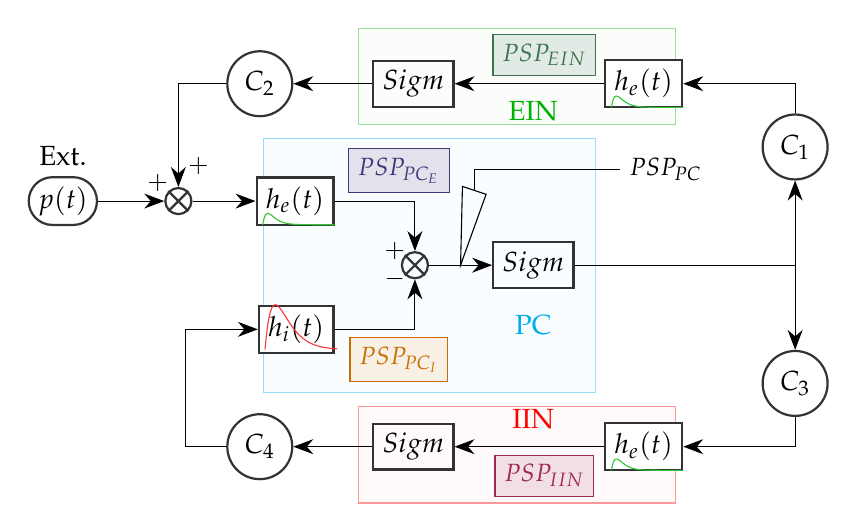
\begin{tikzpicture}[
        pc/.style={draw=cyan!80, fill=cyan!5},
        ein/.style={draw=green!80, fill=green!5},
        iin/.style={draw=red!80, fill=red!5},
        pcLabel/.style={font=\small,text=cyan!80},
        einLabel/.style={font=\small,text=green!80},
        iinLabel/.style={font=\small,text=red!80},
        rectNode/.style={draw=black!80, thick},
        roundNode/.style={circle, draw=black!80, thick},
        ]

\pgfdeclarelayer{bg}
\pgfsetlayers{bg,main}
        
 % Nodes
\node[rectNode] (SigmPC) [] {$Sigm$};
\node[rectNode] (SigmEIN) [above left=2cm and 1cm of SigmPC.center]{$Sigm$};
\node[rectNode] (SigmIIN) [below left=2cm and 1cm of SigmPC.center]{$Sigm$};
\node[rectNode] (PSPPC) [right=1.9cm of SigmEIN.east, fill=white]{$h_e(t)$};
\node[rectNode] (PSPPCI) [right=1.9cm of SigmIIN.east, fill=white]{$h_e(t)$};
\node[rectNode] (PSPEIN) [above left= 0.5cm and 2cm of SigmPC.west, fill=white]{$h_e(t)$};
\node[rectNode] (PSPIIN) [below left= 0.5cm and 2cm of SigmPC.west, fill=white]{$h_i(t)$};
\node[rectNode, rounded corners=3mm] (ext) [left=2cm of PSPEIN.west, label={[]:Ext.}]{$p(t)$};
\node (inpIPSP) [left=0.8cm of PSPIIN.west]{};
\node[roundNode] (c1) [above right=1.2cm and 2.5cm of SigmPC.east]{$C_1$};
\node[roundNode] (c2) [left=1cm of SigmEIN.west]{$C_2$};
\node[roundNode] (c3) [below right=1.2cm and 2.5cm of SigmPC.east]{$C_3$};
\node[roundNode] (c4) [left=1cm of SigmIIN.west]{$C_4$};

% add PC
\node[roundNode] (addPC) [left=0.8cm of SigmPC.west]{};
\draw[-, black!80, thick] (addPC.north west) -- (addPC.south east);
\draw[-, black!80, thick] (addPC.north east) -- (addPC.south west);
% add Excitatory
\node[roundNode] (addExc) [left=0.8cm of PSPEIN.west]{};
\draw[-, black!80, thick] (addExc.north west) -- (addExc.south east);
\draw[-, black!80, thick] (addExc.north east) -- (addExc.south west);

% add PC -> Sigm PC -> PSP PC
\draw[-{Stealth[scale=1.5]}] (addPC.east) -- (SigmPC.west)node[coordinate, pos=0.5](measurepoint){};
\draw[-{Stealth[scale=1.5]}] (SigmPC.east) -| (c1.south);
\draw[-{Stealth[scale=1.5]}] (SigmPC.east) -| (c3.north);


% y0 -> C1 -> Sigm EIN
\draw[-{Stealth[scale=1.5]}] (c1.north) |- (PSPPC.east);
\draw[-{Stealth[scale=1.5]}] (PSPPC.west) -- (SigmEIN.east) node[pos=0.4, above=0.1cm, fill=pyratesgreen!15, draw=pyratesgreen, text=pyratesgreen]{\small$PSP_{EIN}$};

% y0 -> C3 -> Sigm IIN
\draw[-{Stealth[scale=1.5]}] (c3.south) |- (PSPPCI.east);
\draw[-{Stealth[scale=1.5]}] (PSPPCI.west) -- (SigmIIN.east) node[pos=0.4, below=0.1cm, draw=pyratesdarkred, fill=pyratesdarkred!15, text=pyratesdarkred]{\small$PSP_{IIN}$};


% Sigm EIN -> c2 -> add EXC
\draw[-{Stealth[scale=1.5]}] (SigmEIN.west) -- (c2.east);
\draw[-{Stealth[scale=1.5]}] (c2.west) -| (addExc.north) node[pos=0.9, right]{\small$+$};
% external -> add EXC
\draw[-{Stealth[scale=1.5]}] (ext.east) -- (addExc.west) node[pos=0.9, above]{\small$+$};

% add EXC -> PSP EIN
\draw[-{Stealth[scale=1.5]}] (addExc.east) -- (PSPEIN.west);
% PSP EIN -> add PC
\draw[-{Stealth[scale=1.5]}, fill=none] (PSPEIN.east) -| (addPC.north) node[pos=1, left]{\small$+$} node[pos=0.4, above=0.1cm, draw=pyratespurple, fill=pyratespurple!15, text=pyratespurple]{\small$PSP_{PC_E}$};

% Sigm IIN -> C4 -> PSP IIN
\draw[-{Stealth[scale=1.5]}] (SigmIIN.west) -- (c4.east);
\draw[-] (c4.west) -| (inpIPSP.center);
\draw[-{Stealth[scale=1.5]}] (inpIPSP.center) -- (PSPIIN.west);
% PSP IIN -> add PC
\draw[-{Stealth[scale=1.5]}, fill=none] (PSPIIN.east) -| (addPC.south) node[pos=1, left]{\small$-$} node[pos=0.4, below=0.1cm, draw=pyratesorange, fill=pyratesorange!10, text=pyratesorange]{\small$PSP_{PC_I}$};

% electrode
\draw (measurepoint.north) -- (-0.9,1)node[coordinate,pos=0.9](a){} -- (-0.6,0.9)node[coordinate, pos=0.5](b){} -- cycle;
\node (signal)[above right=0.05cm and 2.0cm of a]{\small$PSP_{PC}$};
\draw (b.center) |- (signal.west);


\begin{scope}[shift={(PSPPC.south west)}]
      \begin{axis}[yscale=0.03, xscale=0.16,
            axis x line=none,
            axis y line=none,
            domain=0:140,
            samples=1001,
            xticklabels=\empty,
          ]
          \addplot [green!80] {0.325*x*e^(-0.1*x)};
        \end{axis}
\end{scope}

\begin{scope}[shift={(PSPPCI.south west)}]
      \begin{axis}[yscale=0.03, xscale=0.16,
            axis x line=none,
            axis y line=none,
            domain=0:140,
            samples=1001,
            xticklabels=\empty,
          ]
          \addplot [green!80] {0.325*x*e^(-0.1*x)};
        \end{axis}
\end{scope}

\begin{scope}[shift={(PSPEIN.south west)}]
      \begin{axis}[yscale=0.03, xscale=0.16,
            axis x line=none,
            axis y line=none,
            domain=0:140,
            samples=1001,
            xticklabels=\empty,
          ]
          \addplot [green!80] {0.325*x*e^(-0.1*x)};
        \end{axis}
\end{scope}

\begin{scope}[shift={(PSPIIN.south west)}]
      \begin{axis}[yscale=0.12, xscale=0.16,
            axis x line=none,
            axis y line=none,
            domain=0:140,
            samples=1001,
            xticklabels=\empty,
          ]
          \addplot [red!80] {1.1*x*e^(-0.05*x)};
        \end{axis}
\end{scope}

\begin{pgfonlayer}{bg}
        
    \filldraw [fill=cyan!2,draw=cyan!40]
        ($ (PSPEIN.center) + (-0.4,0.8) $)
        rectangle ($ (PSPIIN.center) + (3.8,-0.8) $);
    \node [below=0.2cm of SigmPC, text=cyan]{PC};
    
    \filldraw [fill=green!2,draw=green!40]
        ($ (SigmEIN.north) + (-0.7,0.4) $)
        rectangle ($ (PSPPC.south) + (0.4,-0.2) $);
    \node [above=1.4cm of SigmPC, text=green]{EIN};
    
    
    \filldraw [fill=red!2,draw=red!40]
        ($ (SigmIIN.north) +  (-0.7,0.2) $)
        rectangle ($ (PSPPCI.south) + (0.4,-0.4) $);
    \node [below=1.4cm of SigmPC, text=red]{IIN};
\end{pgfonlayer}

\end{tikzpicture}
\caption{\textbf{Jansen-Rit Block Diagram as implemented in PyRates:} Each population can be clearly identified by one or more afferent PSP-Blocks and a single Sigmoid that calculates the populations output. This approach is more modular and simplifies conceptual understanding while staying mathematically equivalent. However, due to the explicit fourth PSP-Block it gives up the performance boost.
\quad\todo{possibly the backend-graph-optimization takes care of this? maybe check this later on...} }
\label{fig:pyratesJRBlock}
\end{figure}

\subsection{Implementation of the David \& Friston extensions}


\begin{figure}[H]
	\inputminted[mathescape, frame=lines, linenos, fontsize=\footnotesize, baselinestretch=1.2, bgcolor=LightGray, tabsize=4]
	{python3}{Chapters/Chapter_02_Technical_Concepts/code/psp_subpop.py}
	
	\caption{PSP Block with two Sub-populations in PyRates}
\end{figure}

\subsection{Simulating GABA-A Sedatives}

\quad\todo{why does the reduction of $C$ represent inhibition of the whole system  - what is the difference between thalamic regulation (natural sleep, etc) and GABA-A-receptor binding substances (sedation)? }

\todo{do we have other ways of simulating sedatives in the system?}

%! suppress = EscapeUnderscore

\section{Data Analysis}\label{sec:data-analysis}
\todo{explain features of the raw data, postprocessing steps}

%\section{General features of the simulated data}\label{sec:general-features-of-the-simulated-data}
%
%The NMM is configured to simulate data with a step-size of $1 ms$, yielding a $1000 Hz$ signal.
%In its initial state, the system reacts with high-amplitude oscillations to the "disturbance" of the random input.
%However, the signal usually stabilizes quickly and exhibits the expected behaviour.
%Thus, the first few seconds (stabilization-time varies with parameterization) of simulated data
%are always discarded before further analysis.
%When generating data continuously (without re-initialization of the state-variables),
%this problem only occurs once in the very beginning.
%Changing system parameters abruptly during simulation can also result in disturbances and destabilize the
%signal.


\begin{figure}[H]
    \centering
    \begin{tikzpicture}
        \pgfplotsset{
        %% Axis
            scale only axis,
            width=0.4\linewidth,
            height=4cm,
            every axis/.append style={
                line width=1pt,
                tick style={line width=0.8pt},
                %   grid style={dashed, black!20},
                %  grid=major,
            },
%               %% X-Axis
            xmin=-0.1,
            xmax=7,
        }
        \begin{groupplot} [
                group style={
                    group size=2 by 2,
                    vertical sep=12mm,
                    horizontal sep=12mm,
                },
                yticklabel style={
                    /pgf/number format/fixed,
                    /pgf/number format/precision=2
                },
                legend style={nodes={scale=0.8, transform shape}, thin},
                legend image post style={scale=0},
            ]
            \nextgroupplot[ylabel=$mV$, xlabel=$s$]
            \addplot [line width=.5pt,solid, cyan]
            table[x=x,y=y ,col sep=comma]{data/methodology/uncut.csv};
            \legend{\textbf{A)} uncut data};

            \nextgroupplot[xmin=3.0, xlabel=$s$]
            \addplot [line width=.5pt,solid, cyan]
            table[x=x,y=y ,col sep=comma]{data/methodology/uncut.csv};
            \legend{\textbf{B)} cut data};

            \nextgroupplot[xmax=30.0, ylabel=$dB$, xlabel=$Hz$]
            \addplot [line width=.5pt,solid, cyan]
            table[x=x,y=y ,col sep=comma]{data/methodology/psd_welch_jr.csv};
            \legend{\textbf{C)} J-R PSD};

            \nextgroupplot[xmax=30.0, xlabel=$Hz$]
            \addplot [line width=.5pt,solid, cyan]
            table[x=x,y=y ,col sep=comma]{data/methodology/psd_welch_df.csv};
            \legend{\textbf{D)} D\&F PSD};

        \end{groupplot}
    \end{tikzpicture}

    \caption{
        \textbf{Processing of simulated data.} \\
        \textbf{A) \& B):} removing initially unstable signal by cutting off the first $3s$ of the
        data (generated by Simple Jansen-Rit Model with $C=135$.). \\
        \textbf{C) \& D):} Power Spectral Density of Jansen-Rit and David \& Friston Model (Welch's Method)
    }
    \label{fig:initial_oscilations}
\end{figure}
\chapter{Results}\label{ch:results}
Having accomplished \textbf{Goals 1-3} by implementing the $\lambda$-parameter in our model,
we can set our sights on \textbf{Goal 4} and run a simulation session that mimics GA for each of our two implementations.
As established in Sec.~\ref{subsec:implementing-the-effects-of-propofol},
$\lambda$ may vary between 1 and 3 to approximate the effects of clinically relevant propofol concentrations.
A time-course that closely resembles a real concentration-progression during GA seems intuitively desirable,
but this would complicate a structured analysis of the data, since induction, maintenance and emergence from anaesthesia
have a highly asymmetrical concentration development.
While a fully realistic parameter development might be interesting as a next step,
the general properties of our model under the presence of specific
concentrations of a GABA\textsubscript{A}-potentiating agent
are arguably best explored in a systematic fashion, that still follows the general concept of induction and emergence:
A linear rise to peak dosage, followed by a period of maintenance and a linear decay to the initial condition.

%\section{Exploring realistic parameter ranges}\label{sec:simulation-over-the-parameter-space}

When simulating this time-course over the selected parameter space
$ \lambda \in \left[ 1, 3 \right] $ for $\SI{150}{\second}$ (see Fig~\ref{fig:sedation_sim_jr} \textbf{A}),
the following phenomena can be observed:

\newtoggle{drawLocRoc}

\toggletrue{drawLocRoc}
\def\simRunName{JR_SEDATION_150}
\def\simRunTime{151}
\def\locStart{1.1}
\def\locST{10.07}%6.61
\def\locEnd{2.07}
\def\locET{40.38}%18.89
\def\rocStart{2.0}
\def\rocST{112.88}%48.63
\def\rocEnd{1.00}
\def\rocET{144.46}%62.0
\section{Phenomenology of the Basic JR Model}
    In the baseline state ($\lambda = 1$), the JR model produces the expected well-defined alpha-activity
    with a sharp frequency peak at $\SI{11}{\hertz}$ (Fig~\ref{fig:sedation_sim_jr} \textbf{C}).
\newremark{Spectrogram Amplitude}{
    At this point, it should be noted
    that even though the spectrogram (Fig~\ref{fig:sedation_sim_jr} \textbf{C}) appears to contain a frequency range
    from roughly 6--18Hz at the beginning of the simulation,
    this is misleading.
    The extremely high-amplitude 12Hz peak has noisy flanks with low amplitudes
    (compare to Fig.~\ref{fig:jr_psd}, Fig.~\ref{fig:jr_spec}
    and the scaled plots Fig.~\ref{fig:jr_psd_rescaled}, Fig.~\ref{fig:jr_spec_rescaled}),
    which are highlighted by the chosen colormap and value range.
    Their relative contribution to the signal is close to insignificant in this case.
}
    Increasing the simulated propofol levels first leads to the single dominant frequency at $\SI{11}{\hertz} $
    descending towards $\SI{10}{\hertz} $.
    When reaching $\lambda \approx \locStart $,
    there is an onset of heavy oscillations, characterized by dramatically increasing signal amplitude
    with frequencies peaking at around $5, 10, 15$ and $ \SI{20}{\hertz} $,
    but extending up to $\approx \SI{35}{\hertz} $.
    The frequency peaks appear at multiples of the `fundamental` frequency of $\SI{5}{\hertz}$,
    which is a well-known phenomenon in spectral analysis called `harmonics`.
    Further increase of the concentration shifts the base-frequency and its harmonic components' peaks
    slowly towards lower values, preserving their harmonic nature by moving closer to each other.
    This results in added peaks, always closing the gap to $\approx \SI{35}{\hertz} $.
    Additionally, higher values of $\lambda$ appear to linearly decrease the mean signal voltage.
    Another sudden change occurs around $\lambda \approx \locEnd $,
    where the disturbances disappear again,
    with the system having apparently reached a different stable state with very low activity.
    Signal amplitude is drastically reduced, with remaining activity mostly below $\SI{10}{\hertz}$.
    The single dominant frequency has disappeared completely.
    From there on, the mean signal voltage slowly continues to slightly decrease as before,
    however, the frequency distribution appears to have settled.
    After reaching peak dosage at $\lambda = 3.0$, maintaining it for a few seconds has no further effects.
    Subsequent concentration decrease has the expected reverse effects:
    At first only the signal voltage slightly increases,
    then disturbances begin to form again at $\lambda \approx \rocStart$.
    On the return path, effects roughly mirror the induction.
    It takes a few seconds after $\lambda$ returns to its initial value until the initial state is restored.

\begin{figure}[H]
\begin{tikzpicture}
\pgfplotsset{
        %% Axis
            scale only axis,
            width=0.9\linewidth,
            height=3cm,
            every axis/.append style={
                line width=1pt,
                tick style={line width=0.8pt},
                %   grid style={dashed, black!20},
                %  grid=major,
            },
%               %% X-Axis
            xmin=0.899, xmax=65.0,% xmax=38.899,
        }
        \begin{groupplot} [
                group style={
                    group size=1 by 3,
                    vertical sep=2mm,
                    xlabels at=edge bottom,
                    xticklabels at=edge bottom,
                },
                yticklabel style={
                    /pgf/number format/fixed,
                    /pgf/number format/precision=2
                },
                legend style={nodes={scale=0.8, transform shape}, thin},
                legend image post style={scale=0},
                xlabel=$t(s)$
            ]
            \nextgroupplot[ylabel style={align=center}, ylabel=\begin{tiny}decay-time factor\end{tiny}\\ $\lambda$,
                           ymin=1, ymax=3.1, grid style={dashed,black!20}, grid=major]
            \addplot [line width=.5pt,solid, cyan]
            table[x=x,y=y ,col sep=comma]{data/full_sedation_sim/linear_factors.csv};
                \draw [red, dotted] ([xshift=0.0cm]axis cs:0,1.85) -- ([yshift=0.0cm]axis cs:13.6,1.85) ;
                \draw [red, dotted] ([xshift=0.0cm]axis cs:0,2.05) -- ([yshift=0.0cm]axis cs:16.8,2.05) node[near end,
                        above,font=\tiny]{LOC};
                \draw [red, dotted] ([xshift=0.0cm]axis cs:16.8,1) -- ([yshift=0.0cm]axis cs:16.8,2.05);
                \draw [red, dotted] ([xshift=0.0cm]axis cs:13.6,1) -- ([yshift=0.0cm]axis cs:13.6,1.85);

                \draw [green, dotted] ([xshift=0.0cm]axis cs:65.0,1.48) -- ([yshift=0.0cm]axis cs:57.5,1.48) ;
                \draw [green, dotted] ([xshift=0.0cm]axis cs:65.0,1.95) -- ([yshift=0.0cm]axis cs:51.5,1.95) node[near
                       end,above,font=\tiny]{ROC};
                \draw [green, dotted] ([xshift=0.0cm]axis cs:51.5,1) -- ([yshift=0.0cm]axis cs:51.5,1.95);
                \draw [green, dotted] ([xshift=0.0cm]axis cs:57.5,1) -- ([yshift=0.0cm]axis cs:57.5,1.48);
            \legend{\textbf{A)} propofol concentration};

            \nextgroupplot[ylabel=$mV$]
            \addplot [line width=.5pt,solid, cyan]
            table[x=x,y=y ,col sep=comma]{data/full_sedation_sim/linear.csv};

            \legend{\textbf{B)} signal};

            \nextgroupplot[ymin=0, ymax=40,
                            ylabel=$Hz$,
                            height=5cm
            ]
              \addplot graphics [includegraphics cmd=\pgfimage,
        xmin=0.0,%xmin=0.899,
        xmax=65.0,% xmax=38.899,
        ymin=0, ymax=40]
            {data/full_sedation_sim/linear-img0.png};
            \legend{\textbf{C)} spectrogram};

        \end{groupplot}
     \begin{groupplot} [group style={group size=1 by 3,vertical sep=2mm}]
            \nextgroupplot[axis y line=right, ymin=1, ymax=3.1, ylabel=$\sim c_e (\SI{}{\micro\molar})$,
            yticklabels ={0,5,10,20,30}, ytick={1,1.81,2.164,2.558,2.8},
            axis x line=none]
            \nextgroupplot[axis y line=none, axis x line=none]
            \nextgroupplot[axis y line=none, ymin=0, ymax=40,height=5cm,axis x line=none]
        \end{groupplot}

\end{tikzpicture}
\caption{\textbf{Simulation of a sedation in the JR Model}
}\label{fig:sedation_sim_jr}
\end{figure}

\toggletrue{drawLocRoc}
\def\simRunName{DF_SEDATION_150}
\def\simRunTime{151}
\def\locStart{1.85}
\def\locST{33.5} % 16.17
\def\locEnd{2.05}
\def\locET{39.75}%18.72
\def\rocStart{1.95}
\def\rocST{114.72}%49.3
\def\rocEnd{1.5}
\def\rocET{128.81}%55.03
\section{Phenomenology of the DF Extension}\label{subsec:phenomenology-of-the-df-extension}
Section~\ref{subsec:the-david-and-friston-model} introduces the David--Friston model and
    the mixture of slow and fast kinetics within a population.
    This results in an initial frequency spectrum
    that lacks the distinct high-amplitude peak and instead has a wider distribution with far lower amplitude.

\newremark{Spectrogram Amplitude}{
    Fig.~\ref{fig:sedation_sim_jr}c and Fig.~\ref{fig:sedation_sim_df}c have the same
    color-map and amplitude-range.
    In contrast to the spectrogram of the JR-Model,
    the low-amplitude activity is significant from the start here,
    as it makes up the whole baseline signal.
}
    The DF model initially produces a dominant frequency range at $10-20 \SI{}{\hertz} $,
    which slowly shifts towards $ 5-10 \SI{}{\hertz} $ (Fig~\ref{fig:sedation_sim_df} \textbf{C}) when $\lambda$ starts to increase.
    The mean signal voltage concurrently decreases,
    while oscillation-amplitude is maintained (Fig~\ref{fig:sedation_sim_df} \textbf{B}).
    The system appears to be in a stable state until $ \lambda \approx \locStart $,
    where the sudden onset of dramatically
    increasing signal amplitude with strongly pronounced activity below $ \SI{25}{\hertz} $
    creates multiple strong harmonic frequency peaks.
    Unlike in the JR model, the peaks do not exceed  $ \SI{30}{\hertz} $ and the fundamental frequency starts off
    at roughly $\SI{3}{\hertz}$,
    but otherwise the changes to the spectrum are similar to the JR model.
    Further increasing $\lambda$ has the same minimal effects on the disturbed signal
    as the increase had before exiting the stable state.
    The heavy oscillations remain until $\lambda \approx \locEnd $,
    where the dominant frequencies move below $\SI{10}{\hertz}$.
    Continuing, the signal voltage slowly decreases as before,
    however, the frequency distribution appears to have settled.
    Maintaining peak dosage has no further effects.
    Decreasing the simulated propofol levels again first increases the mean signal voltage
    until the stable state dissolves into heavy oscillations around $\lambda \approx \rocStart$.
    The unstable state prevails until $\lambda$ reaches $\approx \rocEnd$.


\begin{figure}[H]
\begin{tikzpicture}
\pgfplotsset{
        %% Axis
            scale only axis,
            width=0.9\linewidth,
            height=3cm,
            every axis/.append style={
                line width=1pt,
                tick style={line width=0.8pt},
                %   grid style={dashed, black!20},
                %  grid=major,
            },
%               %% X-Axis
            xmin=0.899, xmax=65.0,% xmax=38.899,
        }
        \begin{groupplot} [
                group style={
                    group size=1 by 3,
                    vertical sep=2mm,
                    xlabels at=edge bottom,
                    xticklabels at=edge bottom,
                },
                yticklabel style={
                    /pgf/number format/fixed,
                    /pgf/number format/precision=2
                },
                legend style={nodes={scale=0.8, transform shape}, thin},
                legend image post style={scale=0},
                xlabel=$t(s)$
            ]
            \nextgroupplot[ylabel style={align=center}, ylabel=\begin{tiny}decay-time factor\end{tiny}\\ $\lambda$,
                           ymin=1, ymax=3.1, grid style={dashed,black!20}, grid=major]
            \addplot [line width=.5pt,solid, cyan]
            table[x=x,y=y ,col sep=comma]{data/full_sedation_sim/linear_factors.csv};
                \draw [red, dotted] ([xshift=0.0cm]axis cs:0,1.85) -- ([yshift=0.0cm]axis cs:13.6,1.85) ;
                \draw [red, dotted] ([xshift=0.0cm]axis cs:0,2.05) -- ([yshift=0.0cm]axis cs:16.8,2.05) node[near end,
                        above,font=\tiny]{LOC};
                \draw [red, dotted] ([xshift=0.0cm]axis cs:16.8,1) -- ([yshift=0.0cm]axis cs:16.8,2.05);
                \draw [red, dotted] ([xshift=0.0cm]axis cs:13.6,1) -- ([yshift=0.0cm]axis cs:13.6,1.85);

                \draw [green, dotted] ([xshift=0.0cm]axis cs:65.0,1.48) -- ([yshift=0.0cm]axis cs:57.5,1.48) ;
                \draw [green, dotted] ([xshift=0.0cm]axis cs:65.0,1.95) -- ([yshift=0.0cm]axis cs:51.5,1.95) node[near
                       end,above,font=\tiny]{ROC};
                \draw [green, dotted] ([xshift=0.0cm]axis cs:51.5,1) -- ([yshift=0.0cm]axis cs:51.5,1.95);
                \draw [green, dotted] ([xshift=0.0cm]axis cs:57.5,1) -- ([yshift=0.0cm]axis cs:57.5,1.48);
            \legend{\textbf{A)} propofol concentration};

            \nextgroupplot[ylabel=$mV$]
            \addplot [line width=.5pt,solid, cyan]
            table[x=x,y=y ,col sep=comma]{data/full_sedation_sim/linear.csv};

            \legend{\textbf{B)} signal};

            \nextgroupplot[ymin=0, ymax=40,
                            ylabel=$Hz$,
                            height=5cm
            ]
              \addplot graphics [includegraphics cmd=\pgfimage,
        xmin=0.0,%xmin=0.899,
        xmax=65.0,% xmax=38.899,
        ymin=0, ymax=40]
            {data/full_sedation_sim/linear-img0.png};
            \legend{\textbf{C)} spectrogram};

        \end{groupplot}
     \begin{groupplot} [group style={group size=1 by 3,vertical sep=2mm}]
            \nextgroupplot[axis y line=right, ymin=1, ymax=3.1, ylabel=$\sim c_e (\SI{}{\micro\molar})$,
            yticklabels ={0,5,10,20,30}, ytick={1,1.81,2.164,2.558,2.8},
            axis x line=none]
            \nextgroupplot[axis y line=none, axis x line=none]
            \nextgroupplot[axis y line=none, ymin=0, ymax=40,height=5cm,axis x line=none]
        \end{groupplot}

\end{tikzpicture}
\caption{\textbf{Simulation of a sedation in the DF Model}
}\label{fig:sedation_sim_df}
\end{figure}

\section{Similarities and Differences}
    Both models share some key features during these simulations.
    Three distinguishable states can be observed.
    The initial stable state is followed by a state that is defined by strong harmonic frequencies and dramatically
    increased signal amplitude.
    From there, the system transitions into a low-power state with low frequencies,
    which seems to be mostly saturated and changes little with further increase of decay-time.
    On the return path the second state is visited again before reentering into the initial state.
    Induction and emergence are asymmetrical, even if only marginally so in the JR model.
    The second state can be regarded as the phase transition between the two stable states.
    The system predicts that the frequency range below $\SI{25}{\hertz}$ receives a temporary amplitude boost during
    these phase transitions, which disappear while the parameter changes continue in the same direction.


There are also a few striking differences between the two simulation sessions:
By design,
the JR model produces exclusively near-sinusoid single-peak alpha-activity in the initial state ($\lambda = 1$),
while the DF model creates a range of alpha- and beta-activity.
The JR model spends significant amounts of the session in the second, high-amplitude state,
while these sections are significantly shorter for the DF model.
Also, in the DF model,
the parameter ranges that cause the two high-amplitude states "LOC" and "ROC" differ decisively.
The "LOC"-transition not only ends at a slightly higher $\lambda$ value ($2.05$) than the start of the
"ROC"-transition ($1.95$).
It also starts far higher ($1.85$) than the "ROC" ends ($1.5$).
Consequently, the "LOC" value-range is far shorter ($\text{length}=0.2$) than the "ROC" range
($\text{length}=0.45$).
In the JR model this effect is present as well, but hardly noticeable,
since the differences are much smaller ($2.07$ vs $2.0$ and $1.1$ vs $1.0$, range-lengths $1.06$ and $1.0$).


\todo{transition into discussion}


\chapter{Discussion}
%\todo{-general structure:\\
%-common goals of steyn-ross and this thesis:\\
%--- capture anaesthetic effect with simple(?) model
%-steyn-ross as "landmark" effects\\
%-own contribution:\\
%--- given the steyn ross model -> to what extend can simpler models capture this\\
%--- first candidate: JR\\
%----- biphasic \& minimal hysteresis\\
%----- limits: ...(maybe kuhlmann reference)\\
%--- this motivated next tier of model-sophistication: DF\\
%----- ...}
The shared objective of Steyn-Ross et al. and this thesis,
is to further understanding of the loss and emergence of consciousness,
by capturing anaesthetic effects in an abstract model of brain activity.
Steyn-Ross at al.\ were able to show,
that their model produces hysteresis and a biphasic effect~\cite{hutt_progress_2011}.
The general question of this thesis was,
whether there are simpler models,
that are able to reproduce these phenomena.
The first and arguably most obvious candidate for this was the widely used Jansen-Rit Model,
which is well known for a wide range of dynamics, despite its simplicity.
Generally, the results do suggest that the basic JR model has intrinsic properties that produce
effects similar to those reported in the neural field model~\cite{hutt_progress_2011}:
the default configuration of the famous 1995 model~\cite{jansen_electroencephalogram_1995}
produces a strong biphasic response (see Fig.~\ref{fig:sedation_sim_jr}),
when increasing the inhibitory decay-time constant.
Also a minor hysteresis can be observed, as the transitions in and out of the `unstable' state are not perfectly
`symmetrical'. \todo{quantify}
The biphasic effect occurs very quickly after increasing the IPSP duration, which may in part be due to the default
parameters lying close to a region that produces what David and Friston call `hypersignals`\cite{david_neural_2003}.

\todo{maybe mention kuhlmann here, their criticism of JR limits}

Given the basic model's inability to output realistic frequency distributions or a pronounced hysteresis,
this motivated the next tier of model sophistication, namely the extension of David \&
Friston\cite{david_neural_2003}.
Their contribution of splitting the populations into subpopulations with different PSP properties,
enables the model to produce signals with much richer frequency distributions.
Indeed, the spectra generated during simulated sedation sessions with the default David-Friston model
(see Fig .\ref{fig:sedation_sim_df}) bear similarities to those observed in
real EEG recordings during general anaesthesia~\cite{purdon_electroencephalogram_2013}.


\todo{describe spectral features}
\todo{describe difference between spectral features of LOC and ROC}
\todo{draw comparison to real EEG spectra during anaesthesia~\cite{purdon_electroencephalogram_2013}}
% comparison to other approaches (COALIA / Kuhlmann)

\subsection{draft: argumentation}
The fact that relatively simple computational models can predict the general frequency dynamics occurring during the
drug-induced loss of consciousness,
invites the speculation that effects such as hysteresis and the biphasic effect observed in real EEG recordings can at
least in part be attributed to universally inherent brain-mechanics on population level.

While the effects observed during these simulations provide little to no specific information about the factors
involved in the emergence of consciousness,
they suggest that abstract population dynamics might play a crucial role in modulating the necessary preconditions.
% LIMITS OF THE MODEL!!!!
While the results of the system are promising, it must always be kept in mind that the spatial abstractions of a
population model are not the only simplification in the system used in this thesis.
Many key-concepts and parameters of the model are strictly rooted in neuro-biological evidence,
but there has also been parameter tuning to match desired outputs (e.g.\ the choice of weights for the subpopulations
in~\cite{david_neural_2003} was ultimately motivated by the resulting frequency-spectra).
The chosen weights do lie well within the plausible ranges [citation-needed],
but should not be considered a given.
\todo{soften this harsh criticism...}
Additionally, studying the generated signal of a single macro-column cannot be used to make dependable
general statements about processes as complex as the loss and emergence of consciousness.
\todo{... the breakdown of stabilty in small columns is however a good indication for the loss of necessary
conditions for consciousness in the system as a whole}
\todo{maybe something like "despite severe limits [...], it is remarkable that the simple model can [...]"}
Some of these concerns can be addressed by "whole-brain" network-models,
which consist of many of these columns, ideally spatially realistically interconnected and with propagation delays
between regions that are further apart.

\subsection{draft: kuhlmann/coalia}
\todo{reference COALIA}
\todo{better lead into kuhlmann: something like `similar motivation with different angle`}
\todo{describe kuhlmann paper in more detail}
Kuhlmann et al.'s~\cite{kuhlmann_neural_2016} efforts to use the basic JR model for depth-of-anaesthesia tracking did
produce encouraging results,
even though they concluded that the model might be too simple for their approach.
They experimented with a slight modification of adding self-inhibition to the IIN population without notable success.
It would be interesting to validate this method with the subpopulation extension used in this thesis,
as is appears to be able to model a rich palette of realistic signal states and frequency distributions.

\section{Outlook}
\incomplete{i'm not happy with this section yet...}
%Modeling the mechanisms related to consciousness remains a challenging task
\todo{possible extension: modeling further dynamic effects of anaesthesia? (which exactly?)}
\todo{How could the model be extended: e.g. more realism by incorporation into a whole-brain system like COALIA, ...}
\todo{Possible practical applications: Depth-Of-Anaesthesia-Tracking ~\cite{kuhlmann_neural_2016}, ...}

The development of models that aim to simulate anaesthesia is not only valuable for consciousness research.
An application like the Depth-Of-Anaesthesia-Tracking that Kuhlmann et al.~\cite{kuhlmann_neural_2016} proposed,
could estimate multiple clinically relevant physiological variables like the PSP amplitude and rate constant
\todo{rephrase}.
When matured, such a system could have advantages that would set it apart from current methods,
which rely on algorithmic evaluation of extracted EEG features.
In practice, anaesthetic agents like propofol are often administered in combination with analgesic (pain-reducing)
agents (e.g.\ remifentanil).
This substantially lowers the concentration requirements for the anaesthetic agent to achieve the same level of
sedative effect,
while also helping to increase the quality of anaesthesia, stabilizing the blood pressure and improving recovery
[citation needed].
\todo{note that current methods might not be able to correctly work with or disentangle the actions and interactions
of multiple drugs }
Being able to model and estimate physiological variables during general anaesthesia
could be a valuable tool for clinical practice.



%----------------------------------------------------------------------------------------
%	THESIS CONTENT - APPENDICES
%----------------------------------------------------------------------------------------

\appendix % Cue to tell LaTeX that the following "chapters" are Appendices

%\chapter{Source Code}\label{ch:source_code}

All Source Code is available on GitHub: \\
\faIcon{github} \url{https://github.com/ffriese/sedation_nmm}
\begin{itemize}
    \item \textcolor{pyratesdarkred}{\faIcon{file-pdf}} Thesis Source Code \textcolor{modernblue}{\LaTeX{}} \\
        \url{https://github.com/ffriese/sedation_nmm/tree/main/thesis}
    \item \textcolor{pyratesdarkred}{\faIcon{bezier-curve}} NMM Source Code \textcolor{modernblue}{\faIcon{python}} \\
        \url{https://github.com/ffriese/sedation_nmm/tree/main/code/nmm}
\end{itemize}


%\chapter{Source Code}\label{ch:source_code}

All Source Code is available on GitHub: \\
\faIcon{github} \url{https://github.com/ffriese/sedation_nmm}
\begin{itemize}
    \item \textcolor{pyratesdarkred}{\faIcon{file-pdf}} Thesis Source Code \textcolor{modernblue}{\LaTeX{}} \\
        \url{https://github.com/ffriese/sedation_nmm/tree/main/thesis}
    \item \textcolor{pyratesdarkred}{\faIcon{bezier-curve}} NMM Source Code \textcolor{modernblue}{\faIcon{python}} \\
        \url{https://github.com/ffriese/sedation_nmm/tree/main/code/nmm}
\end{itemize}

%----------------------------------------------------------------------------------------
%	BIBLIOGRAPHY
%----------------------------------------------------------------------------------------

\printbibliography[heading=bibintoc]

%----------------------------------------------------------------------------------------

\end{document}  
